%!TEX root = ../thesis.tex
%*******************************************************************************
%****************************** Third Chapter **********************************
%*******************************************************************************
\chapter{Predicting \mtb{} drug resistance}
\label{chap:dst}
% **************************** Define Graphics Path **************************
\ifpdf
    \graphicspath{{Chapter3/Figs/Raster/}{Chapter3/Figs/PDF/}{Chapter3/Figs/}}
\else
    \graphicspath{{Chapter3/Figs/Vector/}{Chapter3/Figs/}}
\fi

%=========================================================================
%=========================================================================

\setcounter{section}{-1}
\section{Publication and collaboration acknowledgements}
\label{sec:ch3-acknowledge}

A manuscript comprising the work in this chapter and \autoref{chap:clustering} is currently in preparation. In addition to the acknowledgements in \autoref{sec:ch2-acknowledge} the work not completed by myself in this chapter was the drug susceptibility testing (DST) in the laboratory.

\todo[inline]{need to confirm all of this with collabs once I have received the text outlining the methods}

The DST for the samples from Madagascar was conducted by Marie Sylvianne Rabodoarivelo and Simon Grandjean Lapierre. 

\towrite[inline]{acknowledge the people who did the south african DST}

\towrite[inline]{acknowledge the people who did the birmingham DST}


While I did all bioinformatic work in this chapter, I must acknowledge the excellent guidance I have received. My supervisor Zamin Iqbal who always knows the right questions to ask. Simon Grandjean Lapierre helped conceive of this study, along with Zam, and whose clinical perspective helped keep me grounded in the real world. I would also like to acknowledge the many insightful conversations with our other collaborators: Marie Sylvianne Rabodoarivelo, Anastasia Koch, Niaina Rakotosamimanana, Anzaan Dippenaar, and Helen Cox. 

%=========================================================================
\section{Introduction}
Antimicrobial resistance (AMR) predictions from Illumina whole-genome sequencing (WGS) data are now routine for \mtb{} infections in an increasing number of public health agencies. In particular, a WGS-based susceptible prediction for first-line drugs - isoniazid, rifampicin, ethambutol, and pyrazinamide - is now considered accurate enough for clinical use \cite{cryptic2018}. However, being a relatively new sequencing modality, \ont{} has yet to see such large-scale validation.

As discussed in \autoref{chap:clustering}, Illumina WGS is not readily available or feasible in many high-burden tuberculosis (TB) settings. However, \ont{} sequencing is proving to be a useful alternative is such contexts \cite{Inzaule2021,faria2016,quick2016,who-ngs2018}. 

Only two \mtb{} AMR prediction tools - TB-Profiler \cite{phelan2019} and Mykrobe \cite{hunt2019} - have reported results for, and support, \ont{} data; albeit with small sample sizes ($n=3$ and 5 respectively). A recent study from the New York State Department of Health is the largest validation of \ont{} AMR predictions to date, assessing 431 samples. However, they use in-house custom scripts and mutation catalogues, which is unsuitable for general use. 

The software package Mykrobe provides AMR predictions and lineage classification for \mtb{} - amongst other species. It has been validated for Illumina WGS on a comprehensive global cohort and uses a mutation catalogue (panel) that aggregates curated resistance- and susceptibility-associated variants from multiple sources \cite{hunt2019}. However, as mentioned above, \mykrobe{} has only been validated on five \ont{} samples.

The first aim of this chapter is to test \ont{}-based AMR predictions from \mykrobe{} with a larger sample size. For a subset of the data used in \autoref{chap:clustering}, culture-based drug susceptibility testing (DST) phenotypes are available. This phenotyping method is still considered the gold-standard for determining the phenotype of a sample and provides an unbiased truth to detect any sequencing modality-driven differences in WGS-based phenotypes. As our dataset does not have DST information for all samples, or even for all 11 drugs \mykrobe{} provides predictions for, we aim to investigate the concordance of \ont{} with Illumina predictions also. In both cases, we demonstrate that \ont{} provides consistent AMR predictions with Illumina.

One acknowledged limitation of \mykrobe{} and all other \mtb{} AMR prediction tools is that they do not detect off-catalogue (novel) mutations. That is, they cannot detect mutations in resistance-associated genes that do not appear in the catalogue used by the tool. However, a recent study from the \cryptic{} Consortium showed that classifying such novel mutations as "unknown" can improve the pan-susceptibility prediction for first-line drugs \cite{cryptic2018}. 

To this end, we develop and evaluate a genome graph-based \mtb{} AMR prediction software tool, \drprg{}, which can produce these unknown predictions when off-catalogue mutations are detected. We use the methods and understanding developed in \autoref{chap:denovo} and \autoref{chap:clustering} to build a \mtb{} \prg{} for AMR-associated genes and genotype mutations with \pandora{}. In particular, we use the \denovo{} variant discovery functionality of \pandora{} developed in \autoref{chap:denovo} to identify off-catalogue mutations and evaluate how these impact AMR predictions. We show that the novel variants discovered by \drprg{} are precise and reduce the number of missed resistance calls.

%=========================================================================
\section{Dataset}

The \mtb{} samples used in this chapter are those described in \autoref{sec:ch2-dataset}. We use the 150 samples that passed quality control (\autoref{sec:ch2-qc}).

\subsection{Drug susceptibility testing}
\label{sec:dst-methods}

\towrite[inline]{waiting for text from collaborators}

\subsubsection{Madagascar}
\towrite[inline]{summarise supp. extended methods}

See \autoref{app:dst-ext-methods} for full methods.

\noindent
In total, 128 samples have phenotypic information for at least one drug, with 80 having phenotypes for eight drugs. \autoref{tab:available-dst} shows the number of samples with culture-based DST for each drug, and \autoref{fig:available-dst} depicts the combinations of drugs available for samples. For instance, in \autoref{fig:available-dst}, the third column reveals that 29 samples have phenotype information for ofloxacin and amikacin. At the same time, row three shows that 51 samples have available DST for kanamycin. 

Although line probe assay (LPA) results are also available for many samples, we base our phenotype concordance analysis on the culture-based DST data. However, we do use the LPA information to inform reasons for possible errors with resistance prediction. \autoref{tab:full-dst} and \autoref{fig:full-dst} in \autoref{app:full-dst} show the full available DST data from both culture-based and LPA methods.

\begin{table}
\centering
\begin{tabular}{|l|c|}
\hline
Drug         & Count \\ \hline
Amikacin     & 88    \\ \hline
Capreomycin  & 51    \\ \hline
Ethambutol   & 90    \\ \hline
Isoniazid    & 98    \\ \hline
Kanamycin    & 51    \\ \hline
Moxifloxacin & 1     \\ \hline
Ofloxacin    & 86    \\ \hline
Pyrazinamide & 1     \\ \hline
Rifampicin   & 91    \\ \hline
Streptomycin & 90    \\ \hline
\end{tabular}
\caption{Culture-based drug susceptibility data available for samples. The counts are the number of samples with phenotype information available for that drug.}
\label{tab:available-dst}
\end{table}

\begin{figure}
\begin{center}
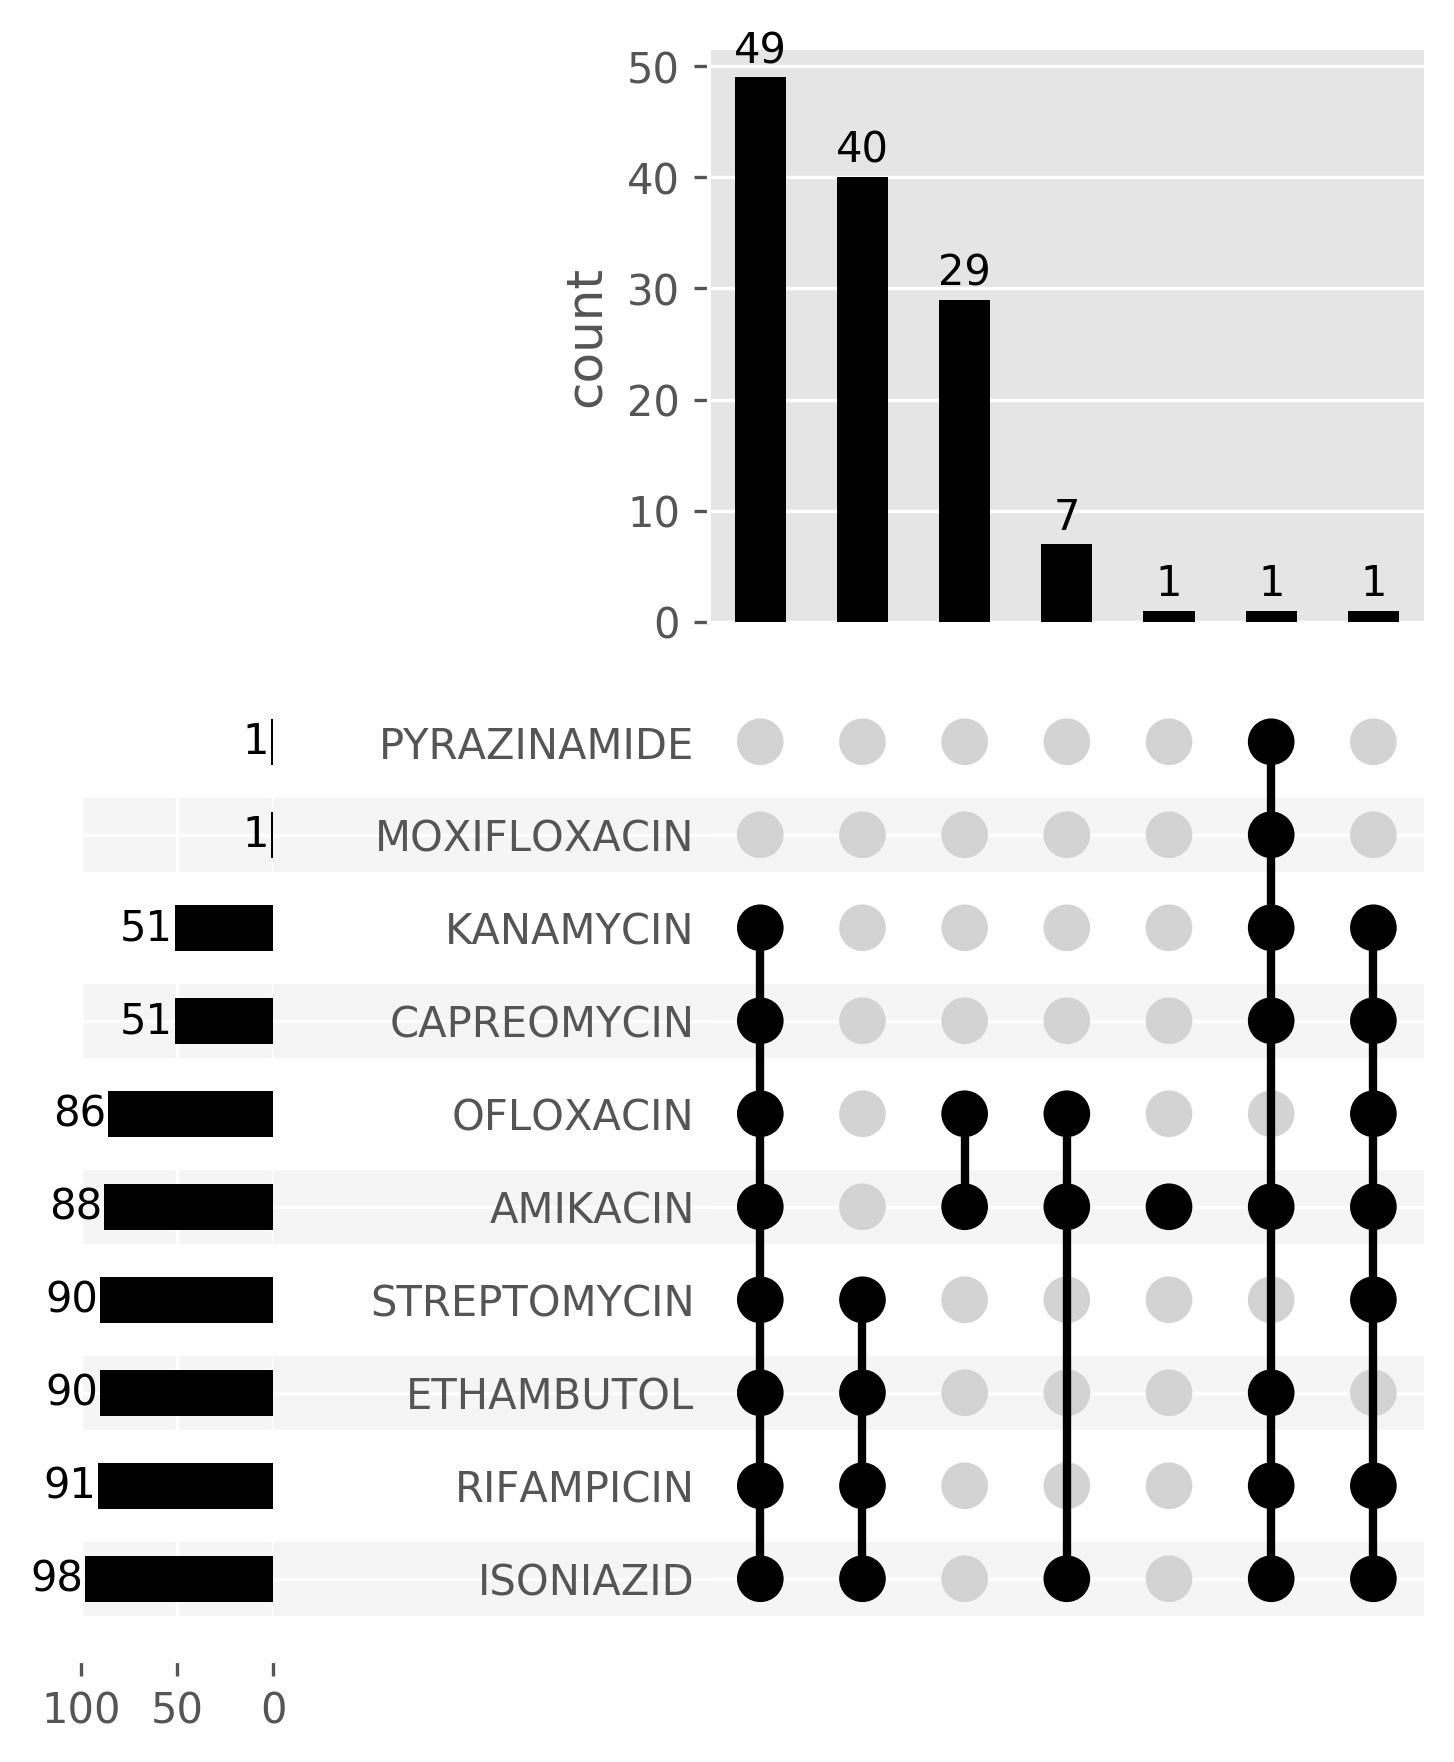
\includegraphics[width=0.90\columnwidth]{Chapter3/Figs/available_dst.png}
\caption{{Culture-based drug susceptibility data available for samples. Each row is a drug, and the columns represent a set of samples with phenotype information for those drugs with a filled cell. The top panel shows the number of samples in the set for that combination of drugs. The bar plot in the left panel shows the number of samples with phenotype information for that drug.
{\label{fig:available-dst}}
}}
\end{center}
\end{figure}
%=========================================================================
\section{Drug resistance prediction with genome graphs}
\label{sec:drprg-methods}

In this section, we describe a method to use genome graphs for predicting drug resistance in \mtb{}; building on previous work in this thesis constructing \mtb{} \prg{}s (\autoref{sec:tbprg}) and calling variants (\autoref{sec:pandora-filters} and \autoref{chap:denovo}). The tool we developed, \drprg{} (Drug Resistance Prediction with Reference Graphs), is written in the Rust programming language and can be found at \url{https://github.com/mbhall88/drprg}.

While tools already exist to predict \mtb{} AMR, the unique component of \drprg{} is the ability to call novel variants. As the \cryptic{} Consortium recently showed, refusing to predict drug phenotypes in cases where "unknown" mutations are present in the associated target gene can lead to increased detection of pan-susceptibility for first-line drugs \cite{cryptic2018}. However, no tool usable by others was made available in that work, and reproducing the results requires running multiple separate tools and scripts. \drprg{} offers a single program for producing this information.

\drprg{} has two distinct phases. In the first phase, we build an index and \prg{} from a panel (catalogue) of mutations known to cause resistance or susceptibility. Second, we genotype Illumina or \ont{} reads against the \prg{}, and phenotype predictions are made for the drugs in the provided panel.

We now outline these two steps in detail.

\subsection{Constructing a panel reference graph}
\label{sec:drprg-index}

The first stage of predicting drug resistance from \drprg{} is coordinated by the \vrb{build} subcommand. As input, \vrb{build} requires a panel of mutations and a reference genome and annotation. We use the reference and annotation for the \mtb{} strain H37Rv (accession NC\_000962.3) and the default panel used by \mykrobe{} (v0.10.0) \cite{hunt2019}. As \mykrobe{} also builds in common variants which are known to \emph{not} cause resistance, we also add such variants from a recent World Health Organization (WHO) catalogue \cite{whopanel2021}. 

The panel of variants can be either resistance- or susceptibility-associated. Each entry in the panel file describes the gene the variant occurs in, the mutation it causes, and any drug it impacts. The mutation can represent a nucleic or amino acid change and is of the form reference, position, alternate. For example, a DNA mutation, \vrb{A5T}, indicates the reference base, \vrb{A}, at position 5 in the gene, is changed to a \vrb{T}. An \vrb{X} indicates any nucleic or amino acid other than the one listed as the reference. We classify the mutation as resistance-causing if a list of drugs is provided for it.

After loading the panel, we generate a reference sequence for each listed gene using the provided reference genome and annotation. If the optional padding argument is given, we add the provided number of bases to the start and end of each gene sequence; we use 100bo of padding for the work in this chapter.

The next step is to convert the panel into a VCF representation. For protein mutations, we convert the amino acids into their respective DNA forms (all possible codons). We confirm that the reference codon matches the reference sequence at the given position in the gene. Protein coordinates (positions) are carefully converted to nucleic acid-space, taking into account the transcription strand specified in the annotation. DNA mutations are likewise checked against the reference. A VCF entry is then generated for each panel entry using the DNA representation. For protein mutations and DNA mutations with an alternate allele of \vrb{X}, all possible changes (except stop codons) are listed in the entry. \autoref{fig:example-panel} shows an example panel and associated VCF.

Another optional parameter of \drprg{} \vrb{build} is the ability to provide a prebuilt \prg{}. If no prebuilt \prg{} is provided, \drprg{} will construct one from the panel. It does this in a similar fashion to the method described in \autoref{sec:tbprg}. That is, for each VCF entry and alternate allele, we replace the gene reference position(s) with the alternate and combine all such mutated sequences into a single FASTA file. We perform a multiple sequence alignment (MSA) on each file, followed by converting the MSA into a local \prg{} using \makeprg{}. Finally, the resulting local \prg{}s, which represent each gene in the panel, are combined into a single \prg{} and indexed with \pandora{}.

For the work in this chapter, we chose to use a prebuilt, population-based \prg{}, rather than the panel \prg{} constructed by \drprg{}. We chose a prebuilt \prg{} because, in the early stages of testing and developing \drprg{}, we found the panel-based \prg{} density and lack of haplotype information were causing a lot of missed resistance (false negatives). \autoref{app:panel-prg-issues} provides a thorough investigation into these problems with the panel-based \prg{}.

The population-based \prg{} we use is built from the same variants as the sparse \prg{} in \autoref{sec:tbprg} - with an important difference. In \autoref{sec:improve-prg} we discussed a potential improvement for the \prg{} construction process whereby whole haplotypes are applied to a reference sequence. When we constructed the original sparse \prg{} in \autoref{sec:tbprg}, we applied each variant, \emph{in isolation}, to the reference sequence. So, if a sample has 3 variants, we built the \prg{} from the reference sequence, plus 3 mutated versions of that reference (see \autoref{sec:improve-prg} for a detailed example). Instead, for the \prg{} we use in this chapter, we apply \emph{all} variants for a sample in the sparse VCF to the (gene) reference sequence - producing a single (gene) haplotype sequence for that sample. We do this for all genes, and use the same MSA, \makeprg{}, \pandora{} index approach mentioned above (and in \autoref{sec:tbprg}). One major difference being the use of a \makeprg{} prototype (v0.2 - mentioned in \autoref{sec:fw-comp-perf}) with a minimum match length of 5. This prototype, developed by Leandro Ishi, retains information about the clustering of sites for each local \prg{}, allowing for quicker updating of \prg{}s with novel variants (as discussed in \autoref{sec:drprg-predict}).


\subsection{Predicting resistance phenotype}
\label{sec:drprg-predict}

The second and final stage of predicting drug resistance with \drprg{} is the \vrb{predict} routine. It takes an index produced by \drprg{} \vrb{build} (\autoref{sec:drprg-index}) and a file containing sequencing reads (Illumina or \ont{}). One optional parameter of interest for the work in this chapter is the ability to discover novel variants.

If requested, the first stage of \drprg{} \vrb{predict} is novel variant discovery in the sequencing reads with \pandora{} \vrb{discover} (version 0.9.0). This version of \pandora{} differs to the one used in \autoref{chap:clustering} in that it outputs all novel variants into a single file compatible with the \makeprg{} prototype used in \autoref{sec:drprg-index}. Next, \makeprg{} updates the \drprg{} \prg{} with these new variants and the resulting updated \prg{} is indexed with \pandora{}. 

One downside to using a population-based \prg{} as we do, is that unlike the panel-based \prg{}, it does not contain all panel variants. As such, for the work in this chapter, we request novel variant discovery in \drprg{} \vrb{predict}.

The second step of \vrb{predict} is genotyping of the sample's sequencing data against the \prg{} (updated or original depending on if variant discovery is requested) with \pandora{} \vrb{map}. An important part of the genotyping step is that we force \pandora{} to output variant coordinates with respect to the gene reference sequences in the index from \vrb{build}. That way, the resulting genotyped VCF coordinates can be compared to the panel VCF in the index. 

After producing the \pandora{} genotyped VCF, we filter out variants that do not meet the provided filtering criteria. \drprg{} \vrb{predict} allows filtering based on: minimum and maximum read depth, strand bias, minimum genotype confidence, minimum fraction of read support (FRS), and maximum indel size. (See \autoref{sec:pandora-filters} for more information on these fields). For the results presented in this chapter, we use a minimum read depth of 3, a minimum FRS of 70\%, a minimum genotype confidence score of 5, a maximum indel size of 20, and a minimum strand bias of 1\% (i.e., we require at least 1\% of total read depth on both strands). We ignore a variant in all subsequent analyses if it fails any of these filters.

Next, we make resistance predictions from the variants that pass filtering. For each call in the genotyped VCF, we fetch all entries in the panel VCF that have overlapping coordinates. If there are no panel variants that overlap the call and novel variant discovery is requested, we classify all drugs associated with the gene of the present call as "unknown" (`U'). If the call is a null genotype (\vrb{.}), we predict all overlapping panel variants as "failed" (`F').

If the variant call was not deemed unknown or failed in the previous step, we check for a match between the call and a panel allele. To determine whether a match exists, we iterate through each panel allele (including the reference) and extract an overlapping sequence between it and the called sequence. If the panel and called allele start at the same position, this is as simple as trimming both sequences to the shortest length of the two. Otherwise, we extract the subsequence denoted by the intersection between the two allele's intervals if they start at different positions. 

For example, if the called allele, \vrb{AT}, starts at position 4 and the panel allele, \vrb{TG}, starts at position 5, their (half-open) intervals are $[4,6)$ and $[5,7)$ respectively. Thus, the intersection of these two alleles would be $[5,6)$, which yields a matching subsequence of \vrb{T} for both. When the two alleles do not have the same length - e.g., indels - we also track the matching sequences' length relative to the reference allele. That way, when there is more than one panel allele that matches the called allele, we return the allele with the match whose length is closest to the called allele.

We add two annotations to each of the genotyped VCF entries that overlap variants in the panel: \vrb{VARID} and \vrb{PREDICT}. \vrb{VARID} is a list of panel variants the position overlaps, and \vrb{PREDICT} is a prediction for each of those panel variants. If there was a non-reference match between a panel variant and the called allele, and the panel variant is resistance-causing, a resistant prediction is recorded. If there was no match, the prediction is susceptible; unless variant discovery was requested, in which case the prediction is unknown. 

After adding the prediction annotations to each entry in the genotyped VCF, we produce a final prediction report as a JSON file. A prediction is provided for every drug present in the panel, along with the supporting evidence (variant(s)). We generate these predictions by going back through the genotyped VCF and using the \vrb{PREDICT} annotation added in the previous step. When different predictions are present for the same drug, the precedence, in order, is resistant, unknown, failed, and susceptible. \autoref{fig:example-drprg-report} shows an example report.

\noindent
All \drprg{} results in this chapter were generated using the commit \href{https://github.com/mbhall88/drprg/tree/cb4f9b82b5d03de45b8016ae5d54bbce7a8f3a0f}{\vrb{cb4f9b8}}.

\subsection{Computational performance}
\label{sec:drprg-comp-perf}

We compare the peak memory usage and runtime for \drprg{} \vrb{predict} with \mykrobe{} - another genome graph-based AMR predictor. \autoref{fig:predict-comp-perf} shows the computational performance of both tools, split by sequencing technology. On average, \drprg{} is faster than \mykrobe{} for both Illumina and \ont{} and uses less memory. As summarised in \autoref{tab:predict-comp-pref}, \drprg{} has a median CPU time of 111.84s (Illumina) and 178.41s (\ont{}) compared to \mykrobe{}'s 196.90s (Illumina) and 248.81s (\ont{}). For memory usage, \drprg{} had a median peak of 224MB (Illumina) and 345.50MB (\ont{}) compared with \mykrobe{}'s 1193MB (Illumina) and 1195MB (\ont{}). However, these time and memory statistics are more than sufficient for both tools to be comfortably run on a standard laptop. 

Building the \drprg{} population-based \prg{} and index took 174.53s of CPU time and had a peak memory usage of 368MB, which occurred during the \makeprg{} step.

\begin{figure}
\begin{center}
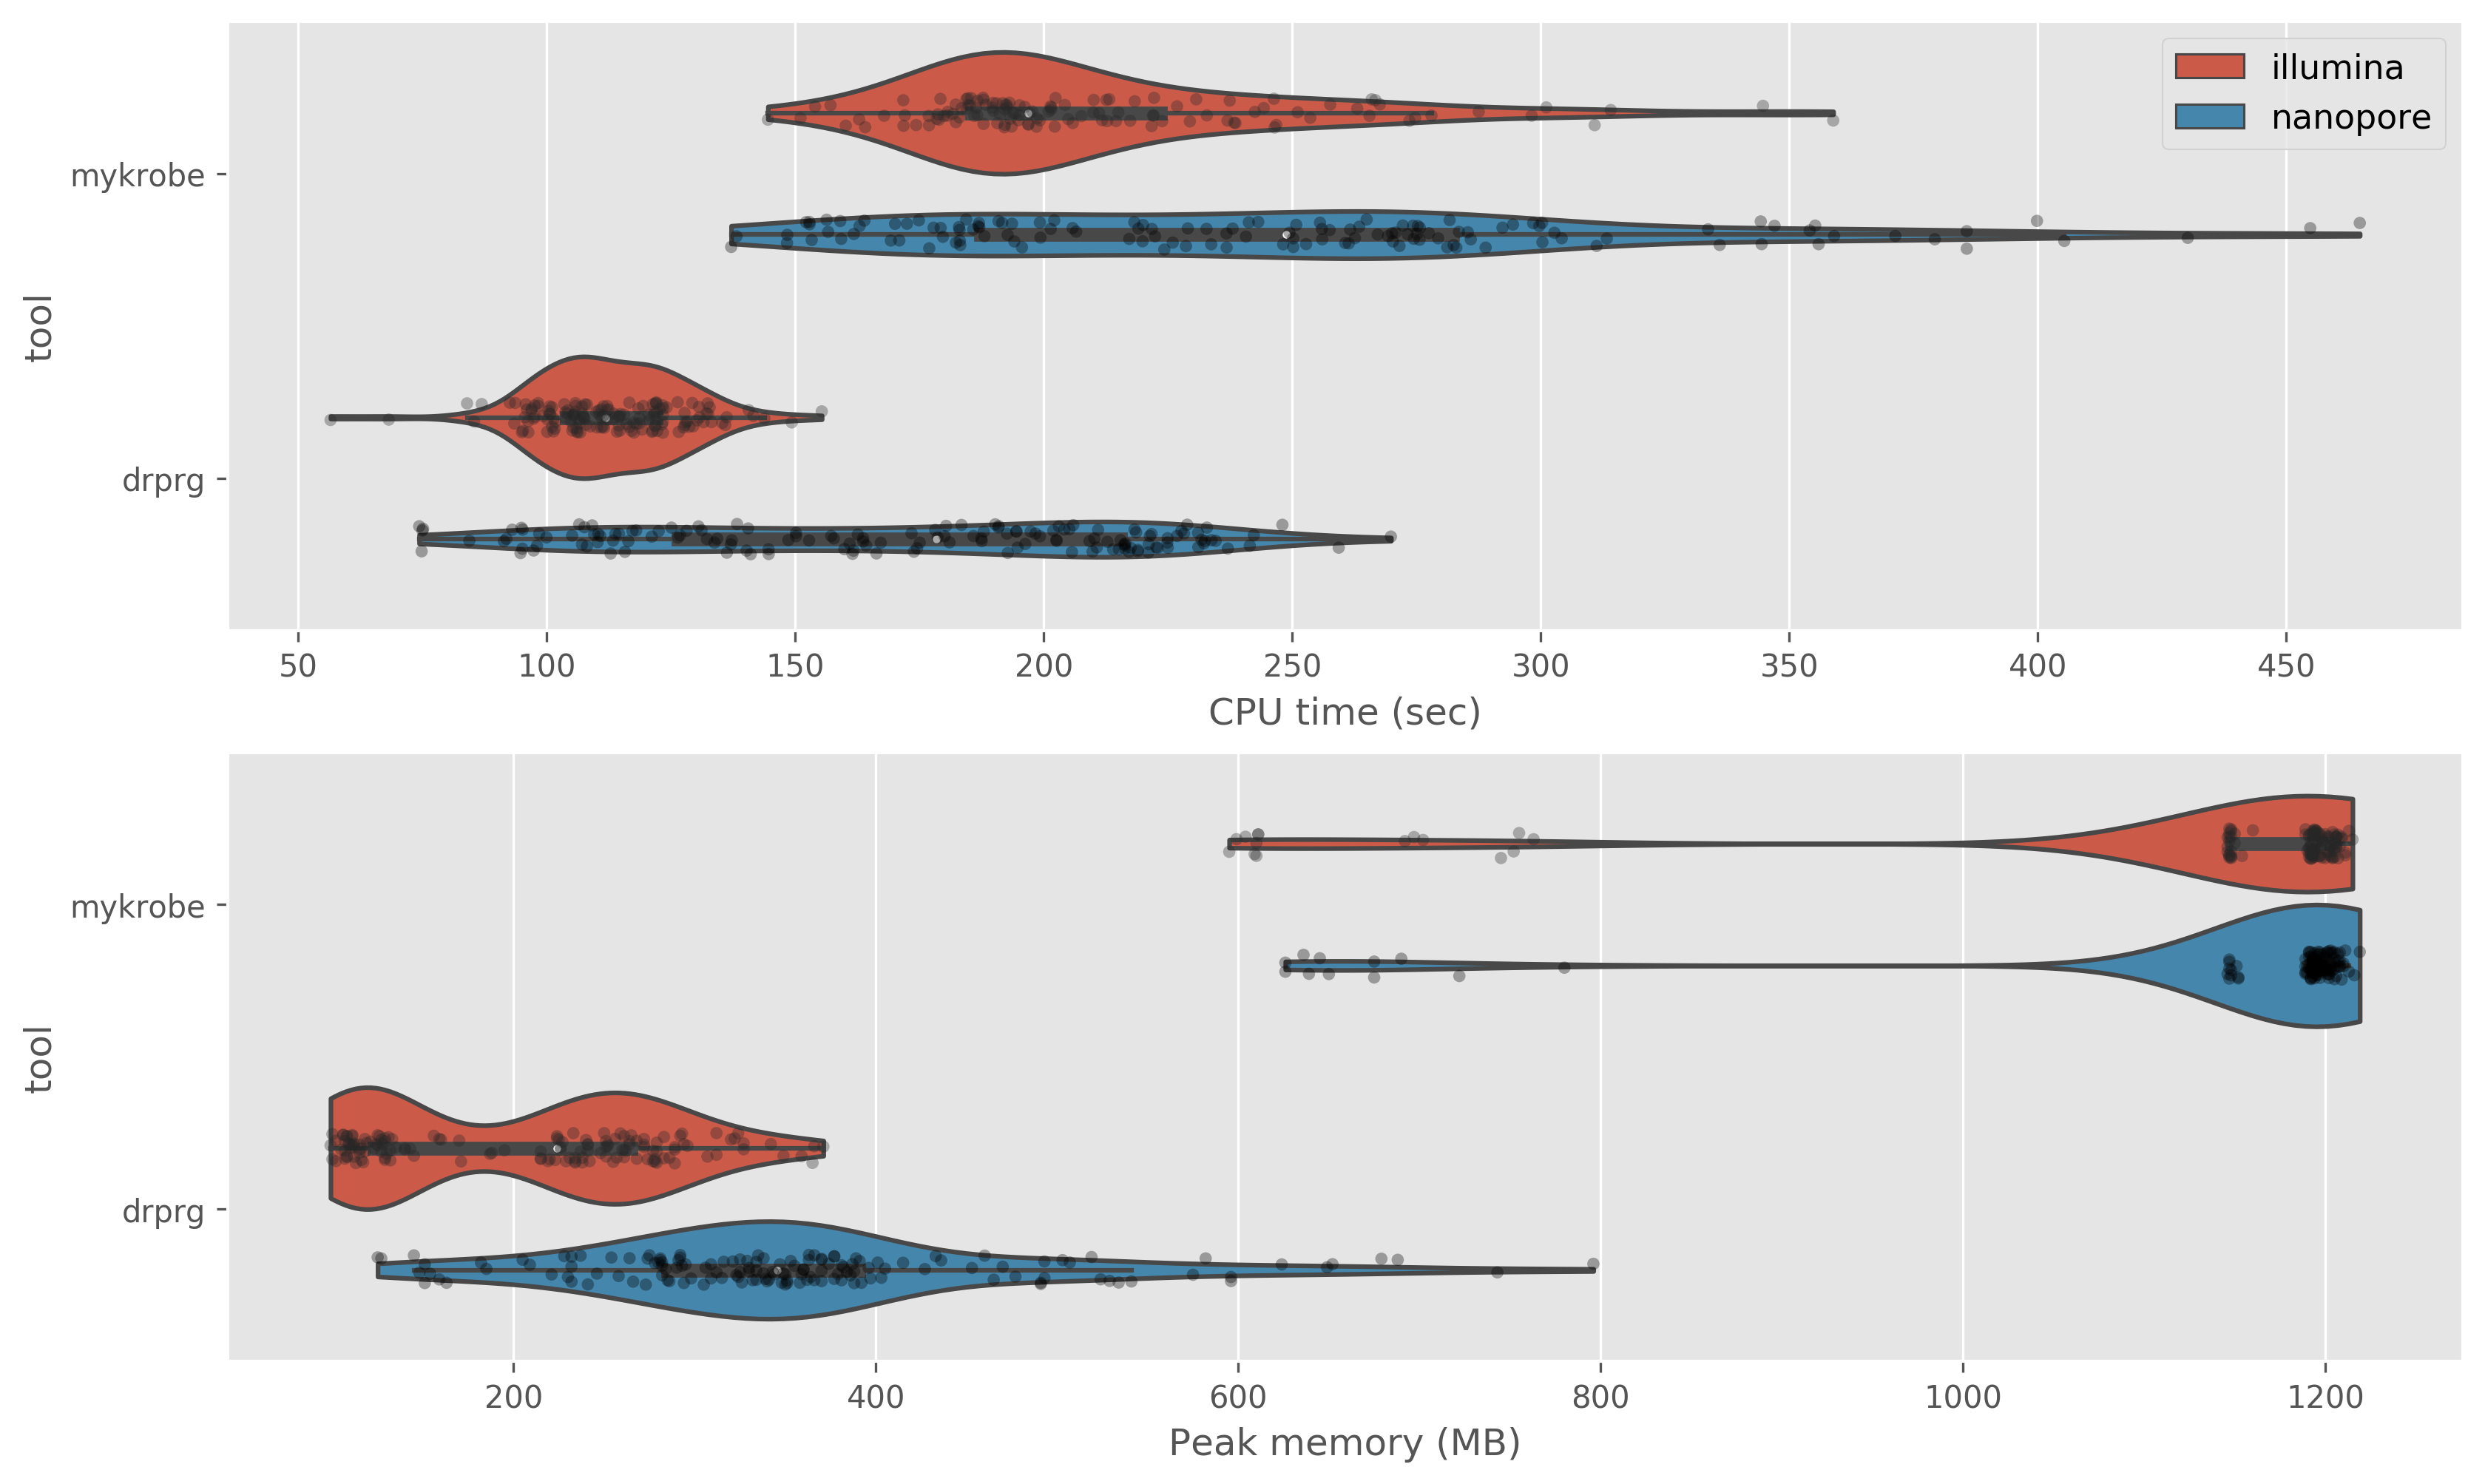
\includegraphics[width=0.90\columnwidth]{Chapter3/Figs/predict-comp-perf.png}
\caption{{The time (seconds; top) and memory (megabytes; bottom) usage of \mykrobe{} and \drprg{} for generating drug resistance predictions. Each tool is additionally split into sequencing technology, with Illumina in red and \ont{} in blue. Data points indicate individual results for a single sample.
{\label{fig:predict-comp-perf}}
}}
\end{center}
\end{figure}


\begin{table}
\centering
\begin{tabular}{|l|l|r|r|r|r|}
\hline
\multicolumn{2}{|l|}{Tool}       & \multicolumn{2}{c|}{\drprg{}} & \multicolumn{2}{c|}{\mykrobe{}} \\ \hline
\multicolumn{2}{|l|}{Technology} & Illumina     & \ont{}    & Illumina      & \ont{}     \\ \hline
\multirow{7}{*}{time (s)}    & mean  & 112.85       & 170.06      & 209.71        & 247.75       \\ \cline{2-6} 
                         & std   & 14.37        & 49.28       & 38.59         & 69.85        \\ \cline{2-6} 
                         & min   & 56.51        & 74.34       & 144.51        & 137.11       \\ \cline{2-6} 
                         & 25\%  & 103.95       & 126.50      & 185.55        & 187.29       \\ \cline{2-6} 
                         & 50\%  & 111.84       & 178.41      & 196.90        & 248.81       \\ \cline{2-6} 
                         & 75\%  & 122.05       & 215.37      & 223.41        & 282.25       \\ \cline{2-6} 
                         & max   & 155.34       & 269.84      & 358.83        & 464.77       \\ \hline
\multirow{7}{*}{memory (MB)}  & mean  & 203.28       & 357.47      & 1126.33       & 1151.14      \\ \cline{2-6} 
                         & std   & 78.64        & 121.38      & 173.29        & 145.87       \\ \cline{2-6} 
                         & min   & 99.00        & 125.00      & 595.00        & 626.00       \\ \cline{2-6} 
                         & 25\%  & 123.25       & 285.25      & 1148.50       & 1192.00      \\ \cline{2-6} 
                         & 50\%  & 224.00       & 345.50      & 1193.00       & 1195.00      \\ \cline{2-6} 
                         & 75\%  & 264.75       & 390.50      & 1201.00       & 1201.00      \\ \cline{2-6} 
                         & max   & 371.00       & 796.00      & 1215.00       & 1219.00      \\ \hline
\end{tabular}
\caption{Summary statistics for the CPU time and peak memory usage of drug resistance prediction with \mykrobe{} and \drprg{} for Illumina and \ont{} data. std=standard deviation}
\label{tab:predict-comp-pref}
\end{table}

%=========================================================================
\section{Concordance with culture-based phenotype}
\label{sec:pheno-concordance}

In this section, we assess the capability of \ont{} WGS to provide reliable drug resistance predictions and evaluate our new genome graph-based approach - \drprg{}.

The culture-based DST profiles gathered in \autoref{sec:dst-methods} are considered the true phenotype against which we will appraise the WGS methods. We exclude moxifloxacin and pyrazinamide from this analysis as DST is only available for one sample. \autoref{tab:available-dst} outlines the total number of samples with phenotype information for each drug.

We compare the WGS-based drug resistance predictions from \mykrobe{} (version 0.10.0; \cite{hunt2019}) and \drprg{} for both Illumina and \ont{} data. For the predictions from \mykrobe{}, we altered some default settings as a result of the analysis in \autoref{app:mykrobe-settings}. The Illumina expected error rate was decreased from 0.05 (default) to 0.001, and the preset \ont{} settings were disabled in favour of an expected error rate of 0.08 and disabling minor resistance calls (haploid model). The \drprg{} settings are detailed in \autoref{sec:drprg-predict}. 

For the drug/sample combinations with available culture-based phenotypes, we classify the WGS predictions as follows. True positive (TP) when the prediction and phenotype are both resistant; true negative (TN) when the prediction and phenotype are both susceptible; false positive (FP) when the prediction is resistant but the phenotype is susceptible; false negative (FN) when the prediction is susceptible but the phenotype is resistant. For this phenotype concordance analysis, we ignore failed and unknown resistance calls from \drprg{} and consider them as susceptible (we assess the utility of these features in \autoref{sec:drprg-discover}). Additionally, for \mykrobe{} Illumina predictions, we interpret minor resistance calls (`r') as resistance (`R').

\autoref{fig:pheno-concordance} shows the concordance of WGS predictions with culture-based phenotypes. The left panel illustrates the number of correct and missed resistance calls made by \mykrobe{} and \drprg{} for both Illumina and \ont{} data. In the right panel, we show the number of correct and incorrect susceptibility predictions. \autoref{tab:pheno-concordance} provides the number of FNs and FPs, along with the false-negative rate (FNR), false-positive rate (FPR), positive predictive value (PPV; precision), and negative predictive value (NPV) for each technology/drug combination. 

\begin{figure}
\begin{center}
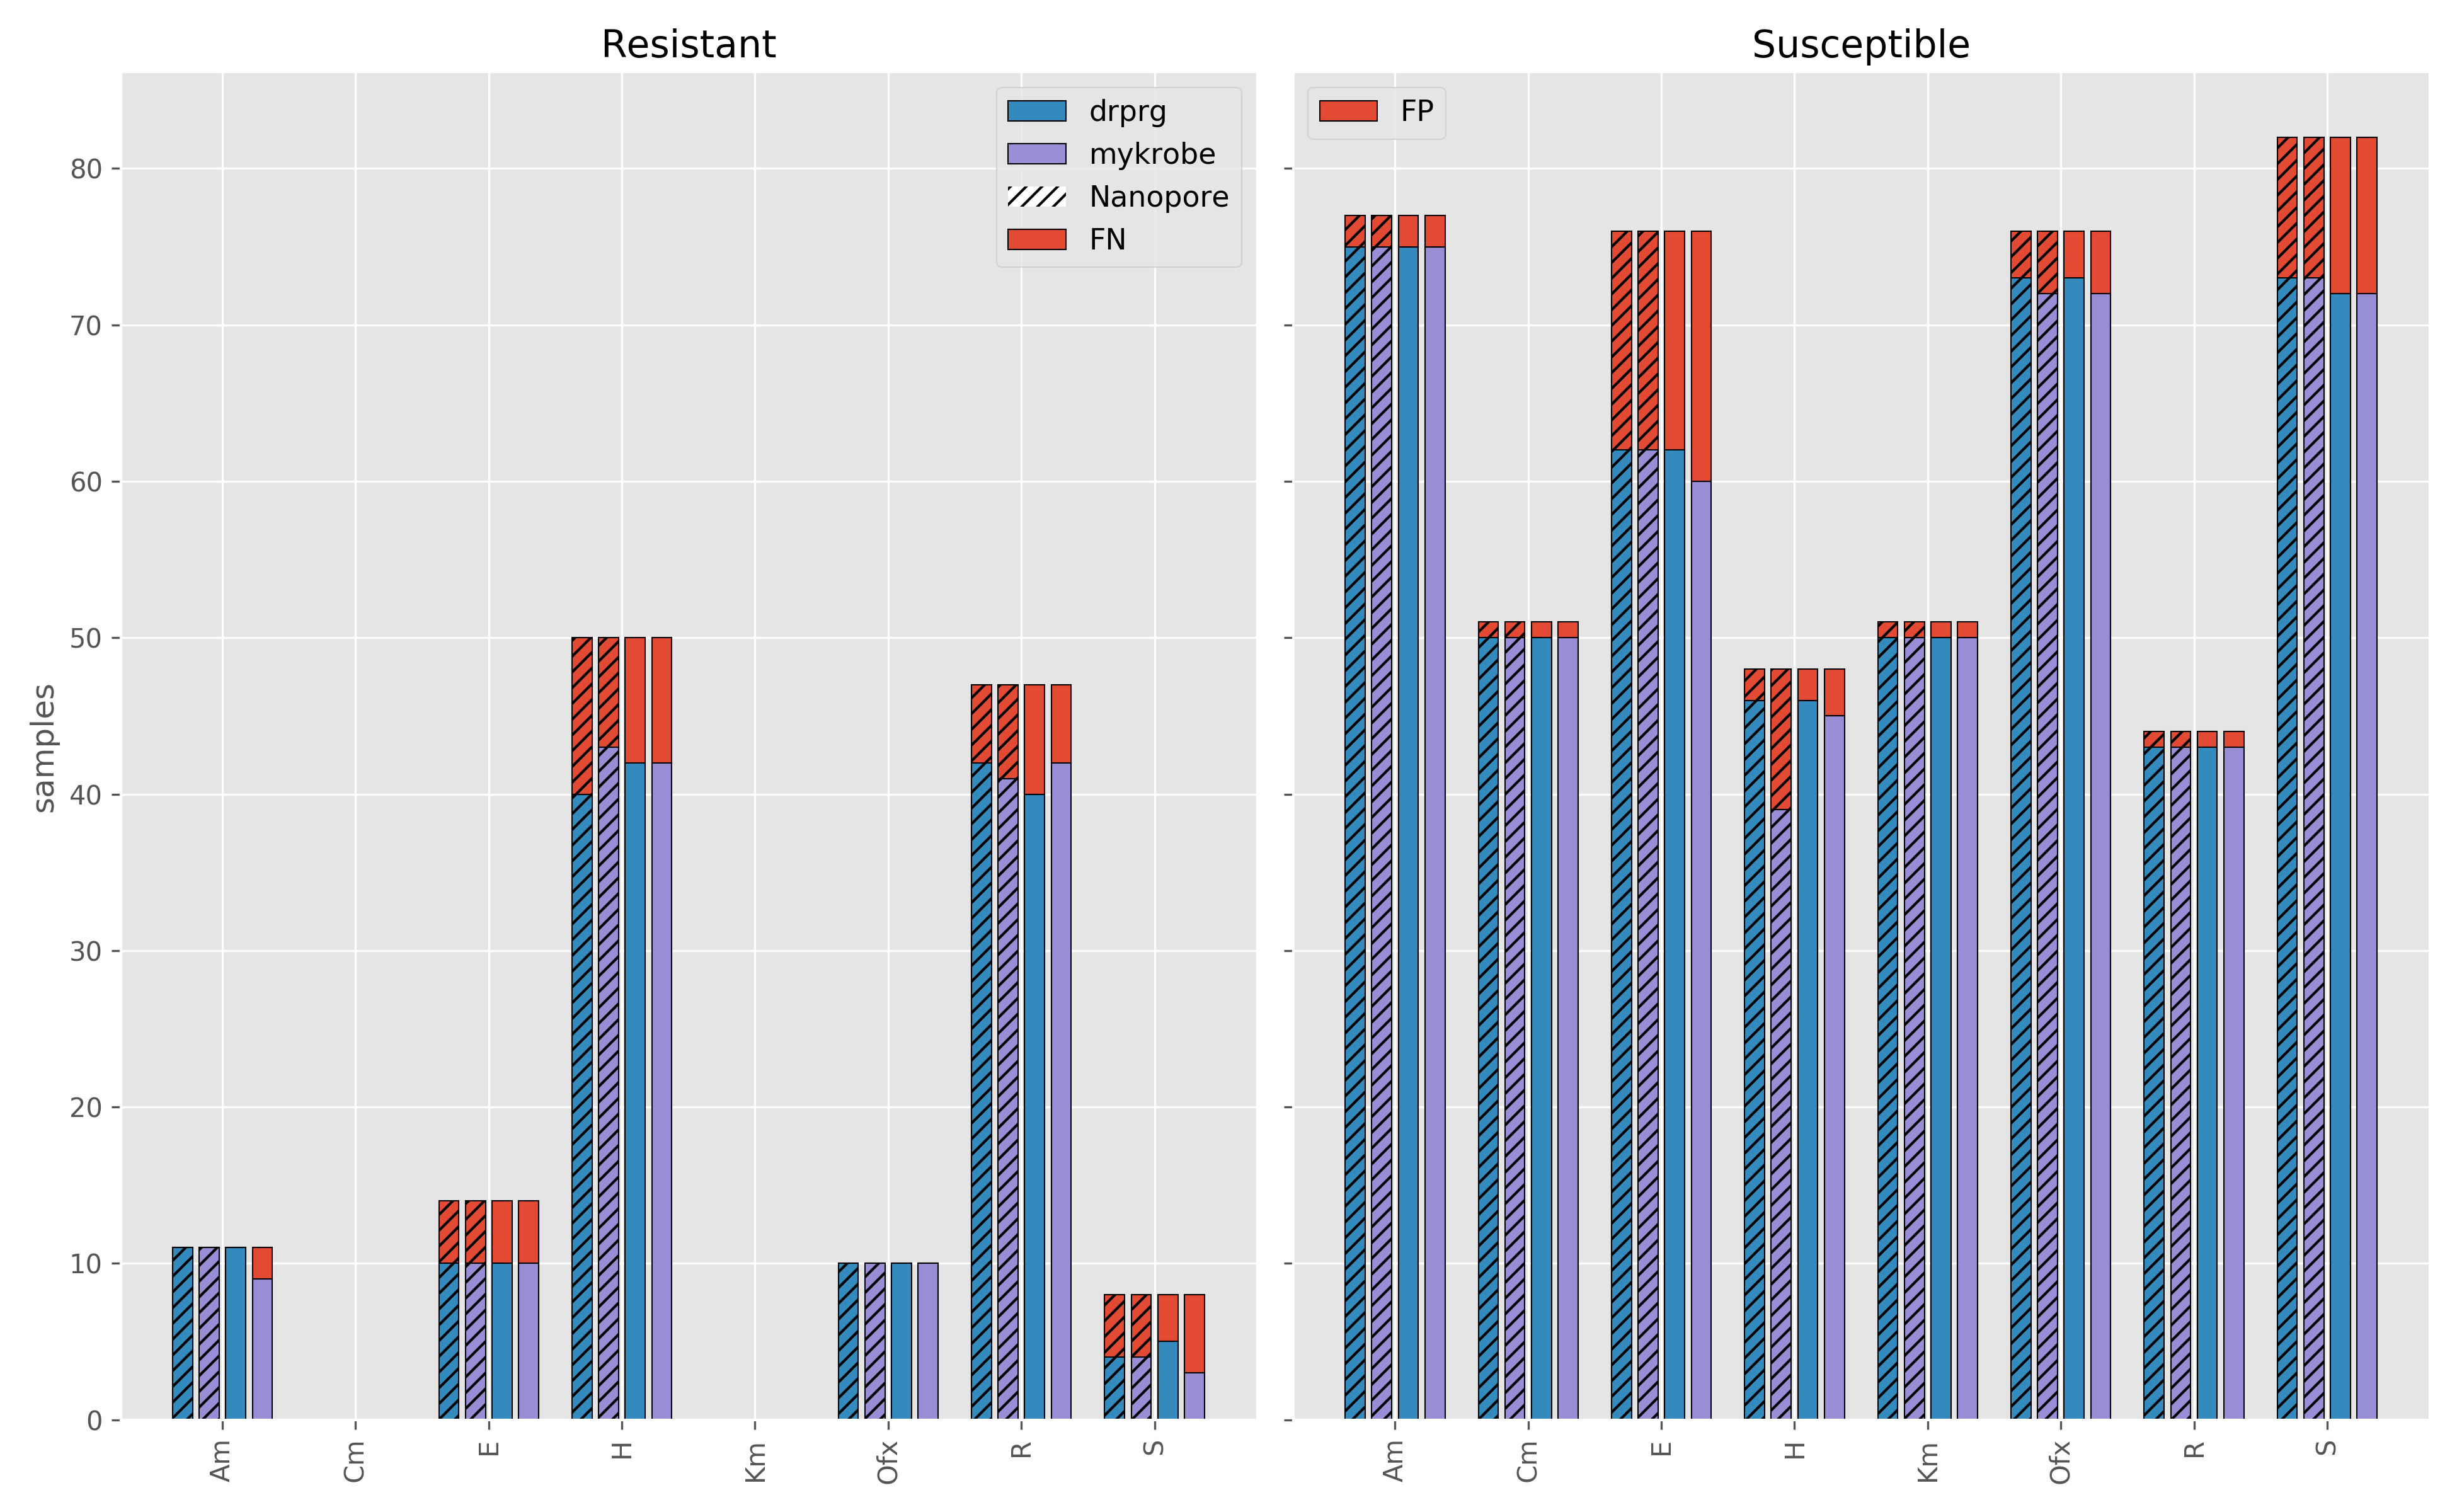
\includegraphics[width=0.90\columnwidth]{Chapter3/Figs/pheno_concordance_plot.png}
\caption{{Number of resistant (left) and susceptible (right) culture-based drug susceptibility testing (DST) phenotypes correctly identified by \mykrobe{} (purple) and \drprg{} (blue) with Illumina (non-striped) and \ont{} (striped) data. The red bars indicate missed (FN) or incorrect (FP) predictions. The x-axis shows the drugs with available phenotype data. E - ethambutol; H - isoniazid; R - rifampicin; S - streptomycin; Km - kanamycin; Am - amikacin; Ofx - ofloxacin; Cm - capreomycin.
{\label{fig:pheno-concordance}}
}}
\end{center}
\end{figure}

These results provide a positive outcome for both our aims. First, \ont{} predictions (striped bars in \autoref{sec:pheno-concordance}) are highly congruent with Illumina. That is, they have equivalent numbers for each classification category. One exception to this is \mykrobe{} \ont{} having noticeably more FPs for isoniazid compared with its Illumina equivalent; all of the extra \ont{} FP calls were indels with no Illumina support. Second, the genome graph-based approach \drprg{}, developed in this chapter, provides predictions consistent with \mykrobe{} - and in some cases, slightly better. 

Ethambutol and streptomycin had many more FPs and FNs compared to the other drugs for both prediction tools. On further investigation, all ethambutol FPs contain strong evidence for a non-synonymous mutation at codon 306 in \textit{embB}, which is strongly linked to drug resistance \cite{Maningi2017,Srivastava2009,Brossier2015}. Of the 14 samples with FP ethambutol calls (16 for \mykrobe{} Illumina), six additionally had LPA phenotypes. In all cases, the LPA disagreed with the culture-based phenotype (i.e., LPA was resistant and culture was susceptible). In addition, half of the FNs also have LPA phenotypes available, and both of these cases differed from the culture-based phenotype. When taken together, this information would suggest that the culture-based phenotype for ethambutol may be wrong in most of these erroneous cases.

While there is no streptomycin LPA data to check discrepancies against, an interesting observation is that 23/38 (60\%) of ethambutol FPs also had an FP streptomycin prediction. There was no one particular mutation found amongst the streptomycin FPs. However, in all cases, the predicted variant had firm support from the tool and the relevant COMPASS and \bcftools{} VCFs from \autoref{sec:var-calls}. 

The high streptomycin false-negative rate for all tools and technologies is challenging to account for, as we do not know which resistance-causing mutations we are expected to find. However, manual assessment of the prediction VCFs produced by \drprg{}, and the individual calls by \mykrobe{}, show there is evidence for known resistance-causing mutations in 4/6 cases. One of those is the mutation K88M in \textit{rpsL} which is not in our panel but has been linked to drug resistance previously \cite{Smittipat2016}. While the other FNs were filtered out either due to low coverage or strand bias. Given the low number of streptomycin-resistant samples (8) in this dataset, it is inappropriate to make any claims about the ability to detect resistance for this drug here.

The results from our genome graph-based tool \drprg{} are very positive. There were only two drug/technology situations where \drprg{} had more errors than \mykrobe{}; isoniazid/\ont{}, with \drprg{} having 10 FNs and \mykrobe{} 7; rifampicin/Illumina, with \drprg{} having 7 FNs and \mykrobe{} 5. For all other drug/technology combinations, \drprg{} has equivalent, or less, errors compared to \mykrobe{}.

\begin{table}
\centering
\resizebox{\textwidth}{!}{%
\begin{tabular}{|l|l|l|l|l|l|l|l|l|}
\hline
Drug &
  Technology &
  Tool &
  FN(R) &
  FP(S) &
  FNR(95\% CI) &
  FPR(95\% CI) &
  PPV(95\% CI) &
  NPV(95\% CI) \\ \hline
\multirow{4}{*}{Amikacin} &
  \multirow{2}{*}{Illumina} &
  \drprg{} &
  0(11) &
  2(77) &
  0.0\% (0.0-25.9\%) &
  2.6\% (0.7-9.0\%) &
  84.6\% (57.8-95.7\%) &
  100.0\% (95.1-100.0\%) \\ \cline{3-9} 
 &
   &
  \mykrobe{} &
  2(11) &
  2(77) &
  18.2\% (5.1-47.7\%) &
  2.6\% (0.7-9.0\%) &
  81.8\% (52.3-94.9\%) &
  97.4\% (91.0-99.3\%) \\ \cline{2-9} 
 &
  \multirow{2}{*}{Nanopore} &
  \drprg{} &
  0(11) &
  2(77) &
  0.0\% (0.0-25.9\%) &
  2.6\% (0.7-9.0\%) &
  84.6\% (57.8-95.7\%) &
  100.0\% (95.1-100.0\%) \\ \cline{3-9} 
 &
   &
  \mykrobe{} &
  0(11) &
  2(77) &
  0.0\% (0.0-25.9\%) &
  2.6\% (0.7-9.0\%) &
  84.6\% (57.8-95.7\%) &
  100.0\% (95.1-100.0\%) \\ \hline
\multirow{4}{*}{Capreomycin} &
  \multirow{2}{*}{Illumina} &
  \drprg{} &
  0(0) &
  1(51) &
  - &
  2.0\% (0.3-10.3\%) &
  0.0\% (0.0-79.3\%) &
  100.0\% (92.9-100.0\%) \\ \cline{3-9} 
 &
   &
  \mykrobe{} &
  0(0) &
  1(51) &
  - &
  2.0\% (0.3-10.3\%) &
  0.0\% (0.0-79.3\%) &
  100.0\% (92.9-100.0\%) \\ \cline{2-9} 
 &
  \multirow{2}{*}{Nanopore} &
  \drprg{} &
  0(0) &
  1(51) &
  - &
  2.0\% (0.3-10.3\%) &
  0.0\% (0.0-79.3\%) &
  100.0\% (92.9-100.0\%) \\ \cline{3-9} 
 &
   &
  \mykrobe{} &
  0(0) &
  1(51) &
  - &
  2.0\% (0.3-10.3\%) &
  0.0\% (0.0-79.3\%) &
  100.0\% (92.9-100.0\%) \\ \hline
\multirow{4}{*}{Ethambutol} &
  \multirow{2}{*}{Illumina} &
  \drprg{} &
  4(14) &
  14(76) &
  28.6\% (11.7-54.6\%) &
  18.4\% (11.3-28.6\%) &
  41.7\% (24.5-61.2\%) &
  93.9\% (85.4-97.6\%) \\ \cline{3-9} 
 &
   &
  \mykrobe{} &
  4(14) &
  16(76) &
  28.6\% (11.7-54.6\%) &
  21.1\% (13.4-31.5\%) &
  38.5\% (22.4-57.5\%) &
  93.8\% (85.0-97.5\%) \\ \cline{2-9} 
 &
  \multirow{2}{*}{Nanopore} &
  \drprg{} &
  4(14) &
  14(76) &
  28.6\% (11.7-54.6\%) &
  18.4\% (11.3-28.6\%) &
  41.7\% (24.5-61.2\%) &
  93.9\% (85.4-97.6\%) \\ \cline{3-9} 
 &
   &
  \mykrobe{} &
  4(14) &
  14(76) &
  28.6\% (11.7-54.6\%) &
  18.4\% (11.3-28.6\%) &
  41.7\% (24.5-61.2\%) &
  93.9\% (85.4-97.6\%) \\ \hline
\multirow{4}{*}{Isoniazid} &
  \multirow{2}{*}{Illumina} &
  \drprg{} &
  8(50) &
  2(48) &
  16.0\% (8.3-28.5\%) &
  4.2\% (1.2-14.0\%) &
  95.5\% (84.9-98.7\%) &
  85.2\% (73.4-92.3\%) \\ \cline{3-9} 
 &
   &
  \mykrobe{} &
  8(50) &
  3(48) &
  16.0\% (8.3-28.5\%) &
  6.2\% (2.1-16.8\%) &
  93.3\% (82.1-97.7\%) &
  84.9\% (72.9-92.1\%) \\ \cline{2-9} 
 &
  \multirow{2}{*}{Nanopore} &
  \drprg{} &
  10(50) &
  2(48) &
  20.0\% (11.2-33.0\%) &
  4.2\% (1.2-14.0\%) &
  95.2\% (84.2-98.7\%) &
  82.1\% (70.2-90.0\%) \\ \cline{3-9} 
 &
   &
  \mykrobe{} &
  7(50) &
  9(48) &
  14.0\% (7.0-26.2\%) &
  18.8\% (10.2-31.9\%) &
  82.7\% (70.3-90.6\%) &
  84.8\% (71.8-92.4\%) \\ \hline
\multirow{4}{*}{Kanamycin} &
  \multirow{2}{*}{Illumina} &
  \drprg{} &
  0(0) &
  1(51) &
  - &
  2.0\% (0.3-10.3\%) &
  0.0\% (0.0-79.3\%) &
  100.0\% (92.9-100.0\%) \\ \cline{3-9} 
 &
   &
  \mykrobe{} &
  0(0) &
  1(51) &
  - &
  2.0\% (0.3-10.3\%) &
  0.0\% (0.0-79.3\%) &
  100.0\% (92.9-100.0\%) \\ \cline{2-9} 
 &
  \multirow{2}{*}{Nanopore} &
  \drprg{} &
  0(0) &
  1(51) &
  - &
  2.0\% (0.3-10.3\%) &
  0.0\% (0.0-79.3\%) &
  100.0\% (92.9-100.0\%) \\ \cline{3-9} 
 &
   &
  \mykrobe{} &
  0(0) &
  1(51) &
  - &
  2.0\% (0.3-10.3\%) &
  0.0\% (0.0-79.3\%) &
  100.0\% (92.9-100.0\%) \\ \hline
\multirow{4}{*}{Ofloxacin} &
  \multirow{2}{*}{Illumina} &
  \drprg{} &
  0(10) &
  3(76) &
  0.0\% (-0.0-27.8\%) &
  3.9\% (1.4-11.0\%) &
  76.9\% (49.7-91.8\%) &
  100.0\% (95.0-100.0\%) \\ \cline{3-9} 
 &
   &
  \mykrobe{} &
  0(10) &
  4(76) &
  0.0\% (-0.0-27.8\%) &
  5.3\% (2.1-12.8\%) &
  71.4\% (45.4-88.3\%) &
  100.0\% (94.9-100.0\%) \\ \cline{2-9} 
 &
  \multirow{2}{*}{Nanopore} &
  \drprg{} &
  0(10) &
  3(76) &
  0.0\% (-0.0-27.8\%) &
  3.9\% (1.4-11.0\%) &
  76.9\% (49.7-91.8\%) &
  100.0\% (95.0-100.0\%) \\ \cline{3-9} 
 &
   &
  \mykrobe{} &
  0(10) &
  4(76) &
  0.0\% (-0.0-27.8\%) &
  5.3\% (2.1-12.8\%) &
  71.4\% (45.4-88.3\%) &
  100.0\% (94.9-100.0\%) \\ \hline
\multirow{4}{*}{Rifampicin} &
  \multirow{2}{*}{Illumina} &
  \drprg{} &
  7(47) &
  1(44) &
  14.9\% (7.4-27.7\%) &
  2.3\% (0.4-11.8\%) &
  97.6\% (87.4-99.6\%) &
  86.0\% (73.8-93.0\%) \\ \cline{3-9} 
 &
   &
  \mykrobe{} &
  5(47) &
  1(44) &
  10.6\% (4.6-22.6\%) &
  2.3\% (0.4-11.8\%) &
  97.7\% (87.9-99.6\%) &
  89.6\% (77.8-95.5\%) \\ \cline{2-9} 
 &
  \multirow{2}{*}{Nanopore} &
  \drprg{} &
  5(47) &
  1(44) &
  10.6\% (4.6-22.6\%) &
  2.3\% (0.4-11.8\%) &
  97.7\% (87.9-99.6\%) &
  89.6\% (77.8-95.5\%) \\ \cline{3-9} 
 &
   &
  \mykrobe{} &
  6(47) &
  1(44) &
  12.8\% (6.0-25.2\%) &
  2.3\% (0.4-11.8\%) &
  97.6\% (87.7-99.6\%) &
  87.8\% (75.8-94.3\%) \\ \hline
\multirow{4}{*}{Streptomycin} &
  \multirow{2}{*}{Illumina} &
  \drprg{} &
  3(8) &
  10(82) &
  37.5\% (13.7-69.4\%) &
  12.2\% (6.8-21.0\%) &
  33.3\% (15.2-58.3\%) &
  96.0\% (88.9-98.6\%) \\ \cline{3-9} 
 &
   &
  \mykrobe{} &
  5(8) &
  10(82) &
  62.5\% (30.6-86.3\%) &
  12.2\% (6.8-21.0\%) &
  23.1\% (8.2-50.3\%) &
  93.5\% (85.7-97.2\%) \\ \cline{2-9} 
 &
  \multirow{2}{*}{Nanopore} &
  \drprg{} &
  4(8) &
  9(82) &
  50.0\% (21.5-78.5\%) &
  11.0\% (5.9-19.6\%) &
  30.8\% (12.7-57.6\%) &
  94.8\% (87.4-98.0\%) \\ \cline{3-9} 
 &
   &
  \mykrobe{} &
  4(8) &
  9(82) &
  50.0\% (21.5-78.5\%) &
  11.0\% (5.9-19.6\%) &
  30.8\% (12.7-57.6\%) &
  94.8\% (87.4-98.0\%) \\ \hline
\end{tabular}%
}
\caption{Comparison of WGS-based drug resistance prediction concordance with culture-based drug susceptibility testing (DST) phenotypes. For this comparison, we assume the DST phenotype is correct and evaluate the WGS predictions accordingly. \drprg{} and \mykrobe{} are the two tools that provide WGS predictions. FN=false negative; R=number of resistant samples; FP=false positive; S=number of susceptible samples; FNR=false negative rate; FPR=false positive rate; PPV=positive predictive value; NPV=negative predictive value; CI=Wilson score confidence interval}
\label{tab:pheno-concordance}
\end{table}

\subsection{Summary}

WGS-based drug resistance predictions from \ont{} are as reliable as those from Illumina when compared to culture-based DST phenotypes. Additionally, we have shown that genome graphs provide reliable predictions for both Illumina and \ont{} data using our tool \drprg{}.

While there is a seemingly high number of FNs and FPs for some drugs, many of these errors result from a suspect culture-based phenotype or the absence of known resistance-causing mutations in the panel.

%=========================================================================
\section{Concordance with Illumina-based phenotype}
\label{sec:geno-concordance}

We saw in \autoref{sec:pheno-concordance} that \ont{}-derived resistance predictions are in line with those from Illumina when comparing to culture-based phenotypes. As not all samples in our dataset have DST data, and not all samples with DST information have all drugs covered, we explore whether \ont{} predictions are concordant with those from \mykrobe{} with Illumina data - for all drugs. Given the comprehensive validation of \mykrobe{}'s prediction power on Illumina data \cite{hunt2019}, if \ont{} results are concordant, this will go a long way to endorsing its use for AMR prediction. In addition, if the Illumina and \ont{} predictions from \drprg{} are consistent with \mykrobe{}, this is an excellent first validation of the method.

We follow the same classification approach as in \autoref{sec:pheno-concordance}, but assume the Illumina predictions from \mykrobe{} are the true phenotype and compare the \mykrobe{} \ont{} and \drprg{} (both modalities) predictions accordingly. \autoref{fig:geno-concordance} and \autoref{tab:geno-concordance} show the results of this analysis.

Across all drugs, there was 8 FN (missed resistance) calls by \mykrobe{} \ont{}. Seven of those FNs are situations where the Illumina data has called minor resistance - a heterozygous call at a resistance-causing variant. As we use a haploid model for \ont{} (see \autoref{app:mykrobe-settings}), this is unavoidable until a diploid model can be employed. We did attempt to use a diploid model for \ont{}, but found a dramatic increase in the number of FNs and FPs due to indel calls. The remaining \ont{} FN has a culture-based DST phenotype of susceptible for that drug (streptomycin), indicating the Illumina prediction may be incorrect. However, there is support for a resistance-causing variant in the VCFs from \autoref{sec:var-calls} - so the truth is uncertain.

For the \drprg{} \ont{} predictions, there were 32 FNs across all drugs. Ten of these were cases where \mykrobe{} called minor resistance. Similar to \mykrobe{} for \ont{}, \drprg{} employs a haploid model for both Illumina and \ont{}; therefore, heterozygous calls are not possible. Another 14 FNs were called resistance by \drprg{} \ont{}, but the variant was filtered due to low FRS - meaning we call susceptible. All but one of these FRS cases was a promoter mutation C-15X in \textit{fabG1}, a mutation that has been known to cause phenotype discrepancies before \cite{cryptic2018}. A further two FNs were also filtered out due to strand bias. Lastly, five FNs were associated with indel calls in \textit{pncA}; indels are a known systematic problem with \ont{} data \cite{watson2019}.

\drprg{} with Illumina data missed 17 resistance calls compared to \mykrobe{} with Illumina. Ten of these were cases of \mykrobe{} calling minor resistance, as mentioned above. Of the remaining 7 FNs, four were related to indel calls in \textit{pncA}, and three have no evidence in the \drprg{} VCF.

Of the 17 FPs made by \mykrobe{} \ont{}, nine show strong support for the resistance-causing variant in the VCFs from \autoref{sec:var-calls} for both technologies. In each of these cases, the \mykrobe{} results from Illumina also called the variant but filtered it out due to low coverage. A further eight are false-positive isoniazid indel calls made by \ont{} in a GC-rich region of \textit{katG}. Additionally, in 8/17 FPs, the culture-based phenotype supports the \ont{} prediction.

The \drprg{} predictions had 23 and 22 FPs for \ont{} and Illumina data respectively. The one difference being the \ont{} predictions have one more isoniazid FP from a \textit{katG} indel call. 11/23 FPs are associated with indel calls in \textit{pncA} causing a false resistance call for pyrazinamide. Indel calls were also the cause of two FPs for isoniazid (\textit{katG}) and one for rifampicin (\textit{rpoB}). Similar to the \mykrobe{} \ont{} calls, 10 of the \drprg{} FPs showed strong support for the resistance-causing variant in VCFs (\autoref{sec:var-calls}) for both technologies, with the \mykrobe{} results from Illumina having also called the variant, but filtered out due to low coverage. Additionally, in 11 FPs, the culture-based phenotype supports the \drprg{} prediction.


\begin{figure}
\begin{center}
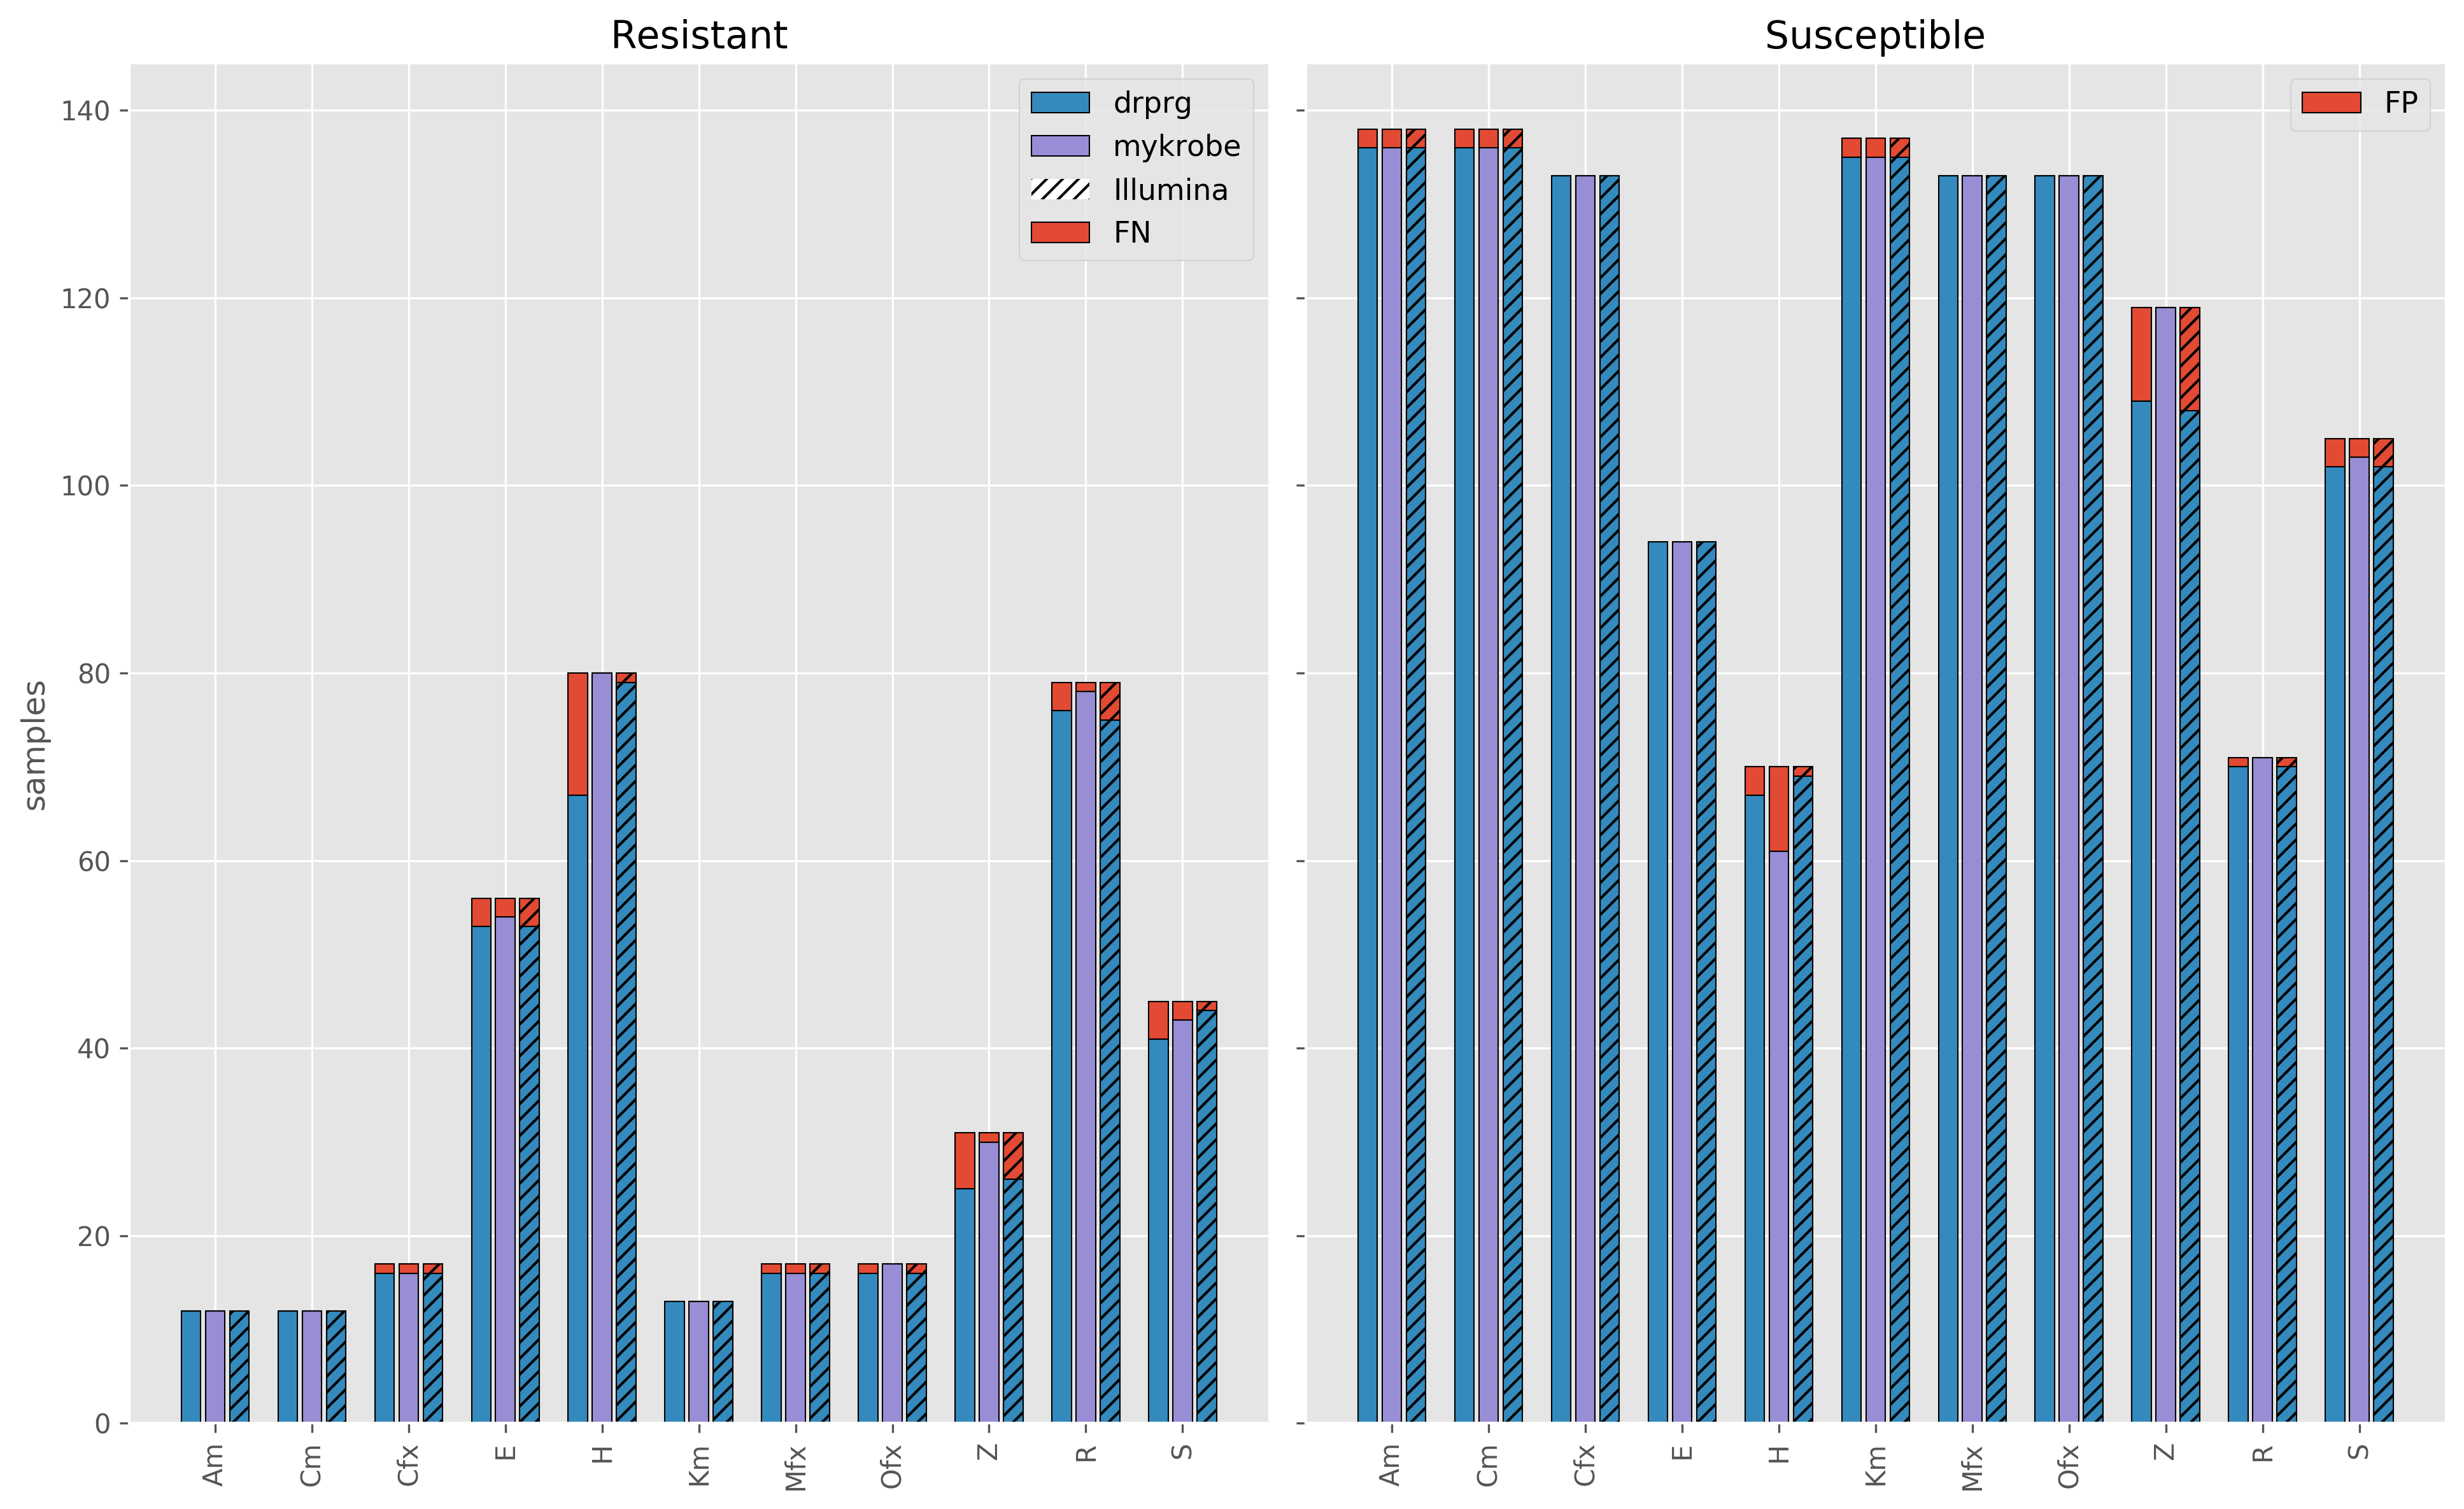
\includegraphics[width=0.90\columnwidth]{Chapter3/Figs/illumina_concordance.png}
\caption{{Number of resistant (left) and susceptible (right) WGS-based drug resistance phenotypes correctly identified by \mykrobe{} \ont{} (purple) and \drprg{} (blue) with Illumina (striped) and \ont{} (non-striped) data. For this analysis, the Illumina-based \mykrobe{} predictions are considered truth and the other predictions are assessed accordingly. The red bars indicate missed (FN) or incorrect (FP) predictions. The x-axis shows the drugs for which \mykrobe{} makes predictions. E - ethambutol; H - isoniazid; Z - pyrazinamide; R - rifampicin; S - streptomycin; Km - kanamycin; Am - amikacin; Ofx - ofloxacin; Cm - capreomycin; Mfx - moxifloxacin.
{\label{fig:geno-concordance}}
}}
\end{center}
\end{figure}

\begin{table}
\centering
\resizebox{\textwidth}{!}{%
\begin{tabular}{|l|l|l|l|l|l|l|l|l|}
\hline
Drug &
  Tool &
  Technology &
  FN(R) &
  FP(S) &
  FNR(95\% CI) &
  FPR(95\% CI) &
  PPV(95\% CI) &
  NPV(95\% CI) \\ \hline
\multirow{3}{*}{Amikacin} &
  \multirow{2}{*}{\drprg{}} &
  Illumina &
  0(12) &
  2(138) &
  0.0\% (0.0-24.2\%) &
  1.4\% (0.4-5.1\%) &
  85.7\% (60.1-96.0\%) &
  100.0\% (97.3-100.0\%) \\ \cline{3-9} 
 &
   &
  \multirow{2}{*}{Nanopore} &
  0(12) &
  2(138) &
  0.0\% (0.0-24.2\%) &
  1.4\% (0.4-5.1\%) &
  85.7\% (60.1-96.0\%) &
  100.0\% (97.3-100.0\%) \\ \cline{2-2} \cline{4-9} 
 &
  \mykrobe{} &
   &
  0(12) &
  2(138) &
  0.0\% (0.0-24.2\%) &
  1.4\% (0.4-5.1\%) &
  85.7\% (60.1-96.0\%) &
  100.0\% (97.3-100.0\%) \\ \hline
\multirow{3}{*}{Capreomycin} &
  \multirow{2}{*}{\drprg{}} &
  Illumina &
  0(12) &
  2(138) &
  0.0\% (0.0-24.2\%) &
  1.4\% (0.4-5.1\%) &
  85.7\% (60.1-96.0\%) &
  100.0\% (97.3-100.0\%) \\ \cline{3-9} 
 &
   &
  \multirow{2}{*}{Nanopore} &
  0(12) &
  2(138) &
  0.0\% (0.0-24.2\%) &
  1.4\% (0.4-5.1\%) &
  85.7\% (60.1-96.0\%) &
  100.0\% (97.3-100.0\%) \\ \cline{2-2} \cline{4-9} 
 &
  \mykrobe{} &
   &
  0(12) &
  2(138) &
  0.0\% (0.0-24.2\%) &
  1.4\% (0.4-5.1\%) &
  85.7\% (60.1-96.0\%) &
  100.0\% (97.3-100.0\%) \\ \hline
\multirow{3}{*}{Ciprofloxacin} &
  \multirow{2}{*}{\drprg{}} &
  Illumina &
  1(17) &
  0(133) &
  5.9\% (1.0-27.0\%) &
  0.0\% (0.0-2.8\%) &
  100.0\% (80.6-100.0\%) &
  99.3\% (95.9-99.9\%) \\ \cline{3-9} 
 &
   &
  \multirow{2}{*}{Nanopore} &
  1(17) &
  0(133) &
  5.9\% (1.0-27.0\%) &
  0.0\% (0.0-2.8\%) &
  100.0\% (80.6-100.0\%) &
  99.3\% (95.9-99.9\%) \\ \cline{2-2} \cline{4-9} 
 &
  \mykrobe{} &
   &
  1(17) &
  0(133) &
  5.9\% (1.0-27.0\%) &
  0.0\% (0.0-2.8\%) &
  100.0\% (80.6-100.0\%) &
  99.3\% (95.9-99.9\%) \\ \hline
\multirow{3}{*}{Ethambutol} &
  \multirow{2}{*}{\drprg{}} &
  Illumina &
  3(56) &
  0(94) &
  5.4\% (1.8-14.6\%) &
  0.0\% (0.0-3.9\%) &
  100.0\% (93.2-100.0\%) &
  96.9\% (91.3-98.9\%) \\ \cline{3-9} 
 &
   &
  \multirow{2}{*}{Nanopore} &
  3(56) &
  0(94) &
  5.4\% (1.8-14.6\%) &
  0.0\% (0.0-3.9\%) &
  100.0\% (93.2-100.0\%) &
  96.9\% (91.3-98.9\%) \\ \cline{2-2} \cline{4-9} 
 &
  \mykrobe{} &
   &
  2(56) &
  0(94) &
  3.6\% (1.0-12.1\%) &
  0.0\% (0.0-3.9\%) &
  100.0\% (93.4-100.0\%) &
  97.9\% (92.7-99.4\%) \\ \hline
\multirow{3}{*}{Isoniazid} &
  \multirow{2}{*}{\drprg{}} &
  Illumina &
  1(80) &
  1(70) &
  1.2\% (0.2-6.7\%) &
  1.4\% (0.3-7.7\%) &
  98.8\% (93.3-99.8\%) &
  98.6\% (92.3-99.7\%) \\ \cline{3-9} 
 &
   &
  \multirow{2}{*}{Nanopore} &
  13(80) &
  3(70) &
  16.2\% (9.7-25.8\%) &
  4.3\% (1.5-11.9\%) &
  95.7\% (88.1-98.5\%) &
  83.8\% (74.2-90.3\%) \\ \cline{2-2} \cline{4-9} 
 &
  \mykrobe{} &
   &
  0(80) &
  9(70) &
  0.0\% (0.0-4.6\%) &
  12.9\% (6.9-22.7\%) &
  89.9\% (81.9-94.6\%) &
  100.0\% (94.1-100.0\%) \\ \hline
\multirow{3}{*}{Kanamycin} &
  \multirow{2}{*}{\drprg{}} &
  Illumina &
  0(13) &
  2(137) &
  0.0\% (0.0-22.8\%) &
  1.5\% (0.4-5.2\%) &
  86.7\% (62.1-96.3\%) &
  100.0\% (97.2-100.0\%) \\ \cline{3-9} 
 &
   &
  \multirow{2}{*}{Nanopore} &
  0(13) &
  2(137) &
  0.0\% (0.0-22.8\%) &
  1.5\% (0.4-5.2\%) &
  86.7\% (62.1-96.3\%) &
  100.0\% (97.2-100.0\%) \\ \cline{2-2} \cline{4-9} 
 &
  \mykrobe{} &
   &
  0(13) &
  2(137) &
  0.0\% (0.0-22.8\%) &
  1.5\% (0.4-5.2\%) &
  86.7\% (62.1-96.3\%) &
  100.0\% (97.2-100.0\%) \\ \hline
\multirow{3}{*}{Moxifloxacin} &
  \multirow{2}{*}{\drprg{}} &
  Illumina &
  1(17) &
  0(133) &
  5.9\% (1.0-27.0\%) &
  0.0\% (0.0-2.8\%) &
  100.0\% (80.6-100.0\%) &
  99.3\% (95.9-99.9\%) \\ \cline{3-9} 
 &
   &
  \multirow{2}{*}{Nanopore} &
  1(17) &
  0(133) &
  5.9\% (1.0-27.0\%) &
  0.0\% (0.0-2.8\%) &
  100.0\% (80.6-100.0\%) &
  99.3\% (95.9-99.9\%) \\ \cline{2-2} \cline{4-9} 
 &
  \mykrobe{} &
   &
  1(17) &
  0(133) &
  5.9\% (1.0-27.0\%) &
  0.0\% (0.0-2.8\%) &
  100.0\% (80.6-100.0\%) &
  99.3\% (95.9-99.9\%) \\ \hline
\multirow{3}{*}{Ofloxacin} &
  \multirow{2}{*}{\drprg{}} &
  Illumina &
  1(17) &
  0(133) &
  5.9\% (1.0-27.0\%) &
  0.0\% (0.0-2.8\%) &
  100.0\% (80.6-100.0\%) &
  99.3\% (95.9-99.9\%) \\ \cline{3-9} 
 &
   &
  \multirow{2}{*}{Nanopore} &
  1(17) &
  0(133) &
  5.9\% (1.0-27.0\%) &
  0.0\% (0.0-2.8\%) &
  100.0\% (80.6-100.0\%) &
  99.3\% (95.9-99.9\%) \\ \cline{2-2} \cline{4-9} 
 &
  \mykrobe{} &
   &
  0(17) &
  0(133) &
  0.0\% (0.0-18.4\%) &
  0.0\% (0.0-2.8\%) &
  100.0\% (81.6-100.0\%) &
  100.0\% (97.2-100.0\%) \\ \hline
\multirow{3}{*}{Pyrazinamide} &
  \multirow{2}{*}{\drprg{}} &
  Illumina &
  5(31) &
  11(119) &
  16.1\% (7.1-32.6\%) &
  9.2\% (5.2-15.8\%) &
  70.3\% (54.2-82.5\%) &
  95.6\% (90.1-98.1\%) \\ \cline{3-9} 
 &
   &
  \multirow{2}{*}{Nanopore} &
  6(31) &
  10(119) &
  19.4\% (9.2-36.3\%) &
  8.4\% (4.6-14.8\%) &
  71.4\% (54.9-83.7\%) &
  94.8\% (89.1-97.6\%) \\ \cline{2-2} \cline{4-9} 
 &
  \mykrobe{} &
   &
  1(31) &
  0(119) &
  3.2\% (0.6-16.2\%) &
  0.0\% (0.0-3.1\%) &
  100.0\% (88.6-100.0\%) &
  99.2\% (95.4-99.9\%) \\ \hline
\multirow{3}{*}{Rifampicin} &
  \multirow{2}{*}{\drprg{}} &
  Illumina &
  4(79) &
  1(71) &
  5.1\% (2.0-12.3\%) &
  1.4\% (0.2-7.6\%) &
  98.7\% (92.9-99.8\%) &
  94.6\% (86.9-97.9\%) \\ \cline{3-9} 
 &
   &
  \multirow{2}{*}{Nanopore} &
  3(79) &
  1(71) &
  3.8\% (1.3-10.6\%) &
  1.4\% (0.2-7.6\%) &
  98.7\% (93.0-99.8\%) &
  95.9\% (88.6-98.6\%) \\ \cline{2-2} \cline{4-9} 
 &
  \mykrobe{} &
   &
  1(79) &
  0(71) &
  1.3\% (0.2-6.8\%) &
  0.0\% (0.0-5.1\%) &
  100.0\% (95.3-100.0\%) &
  98.6\% (92.5-99.8\%) \\ \hline
\multirow{3}{*}{Streptomycin} &
  \multirow{2}{*}{\drprg{}} &
  Illumina &
  1(45) &
  3(105) &
  2.2\% (0.4-11.6\%) &
  2.9\% (1.0-8.1\%) &
  93.6\% (82.8-97.8\%) &
  99.0\% (94.7-99.8\%) \\ \cline{3-9} 
 &
   &
  \multirow{2}{*}{Nanopore} &
  4(45) &
  3(105) &
  8.9\% (3.5-20.7\%) &
  2.9\% (1.0-8.1\%) &
  93.2\% (81.8-97.7\%) &
  96.2\% (90.7-98.5\%) \\ \cline{2-2} \cline{4-9} 
 &
  \mykrobe{} &
   &
  2(45) &
  2(105) &
  4.4\% (1.2-14.8\%) &
  1.9\% (0.5-6.7\%) &
  95.6\% (85.2-98.8\%) &
  98.1\% (93.3-99.5\%) \\ \hline
\end{tabular}%
}
\caption{Comparison of \drprg{} and \mykrobe{} \ont{} drug resistance predictions with \mykrobe{} Illumina predictions. For this comparison, we assume the \mykrobe{} resistance prediction from Illumina data is correct and evaluate the other predictions accordingly. FN=false negative; R=number of resistant samples; FP=false positive; S=number of susceptible samples; FNR=false negative rate; FPR=false positive rate; PPV=positive predictive value; NPV=negative predictive value; CI=Wilson score confidence interval}
\label{tab:geno-concordance}
\end{table}

\subsection{Summary}

In summary, \mykrobe{} \ont{} AMR predictions are consistent with those from Illumina data. There were some discrepancies; however, all but one of the missed resistance calls was due to heterozygous calls, which \ont{} cannot replicate yet. Additionally, many of the false resistance calls were either \ont{} making incorrect indel calls, or Illumina missing variants with strong support from the analysis in \autoref{sec:var-calls}.

For most drugs, \drprg{} predictions are concordant with \mykrobe{}'s Illumina calls. More than half of the \drprg{} missed resistance calls were due to it not being able to detect heterozygous positions. \drprg{} \ont{} predictions also missed some resistant calls because of a low fraction of read support for the mutation in question. The resounding reason for false resistance calls from \drprg{}, for both technologies, was incorrect indel calls in \textit{pncA}. However, nearly half of the \drprg{} false positives are potentially missed resistance on \mykrobe{}'s part due to it having filtered out the calls due to low support. 

%=========================================================================
\section{Effect of \ont{} read depth}
\label{sec:dst-covg}

An important consideration when performing \ont{} sequencing for AMR prediction is how much data is needed. The quantity of data required has implications for how long the \ont{} sequencing device needs to be run or how many samples can be multiplexed in a single run in order to yield sufficient data for reliable predictions. A previous study by Votintseva \etal{} found that deep coverage is required of \ont{} to predict drug resistance accurately\cite{Votintseva2017}. As \ont{} sequencing advances quickly, and our dataset contains a broad \ont{} depth-of-coverage range (29-150x), we explore whether this requirement of high coverage still holds. 

We binned samples into groups based on their read depth. The groups were segregated into lots of 10x depth. That is, if a sample has a read depth of 56, it is assigned to the 50x bin, which covers samples with read depth less than 60, but $\ge50$. We calculate the proportions of each drug resistance classification (FN, TP, TN, FP) present for each bin. For this analysis, we use the culture-based phenotype classifications from \autoref{sec:pheno-concordance}. If low read depth leads to poor resistance prediction, we would expect the proportions of FPs and FNs in the low-depth bins to be greater than in the high-depth bins. 

As \autoref{fig:pheno-covg} illustrates, we see no relationship between \ont{} read depth and erroneous predictions. Further work at depths lower than 30x is warranted, but this is convincing evidence that samples with "only" 30x \ont{} read depth still yield reliable resistance predictions. 

\begin{figure}
\begin{center}
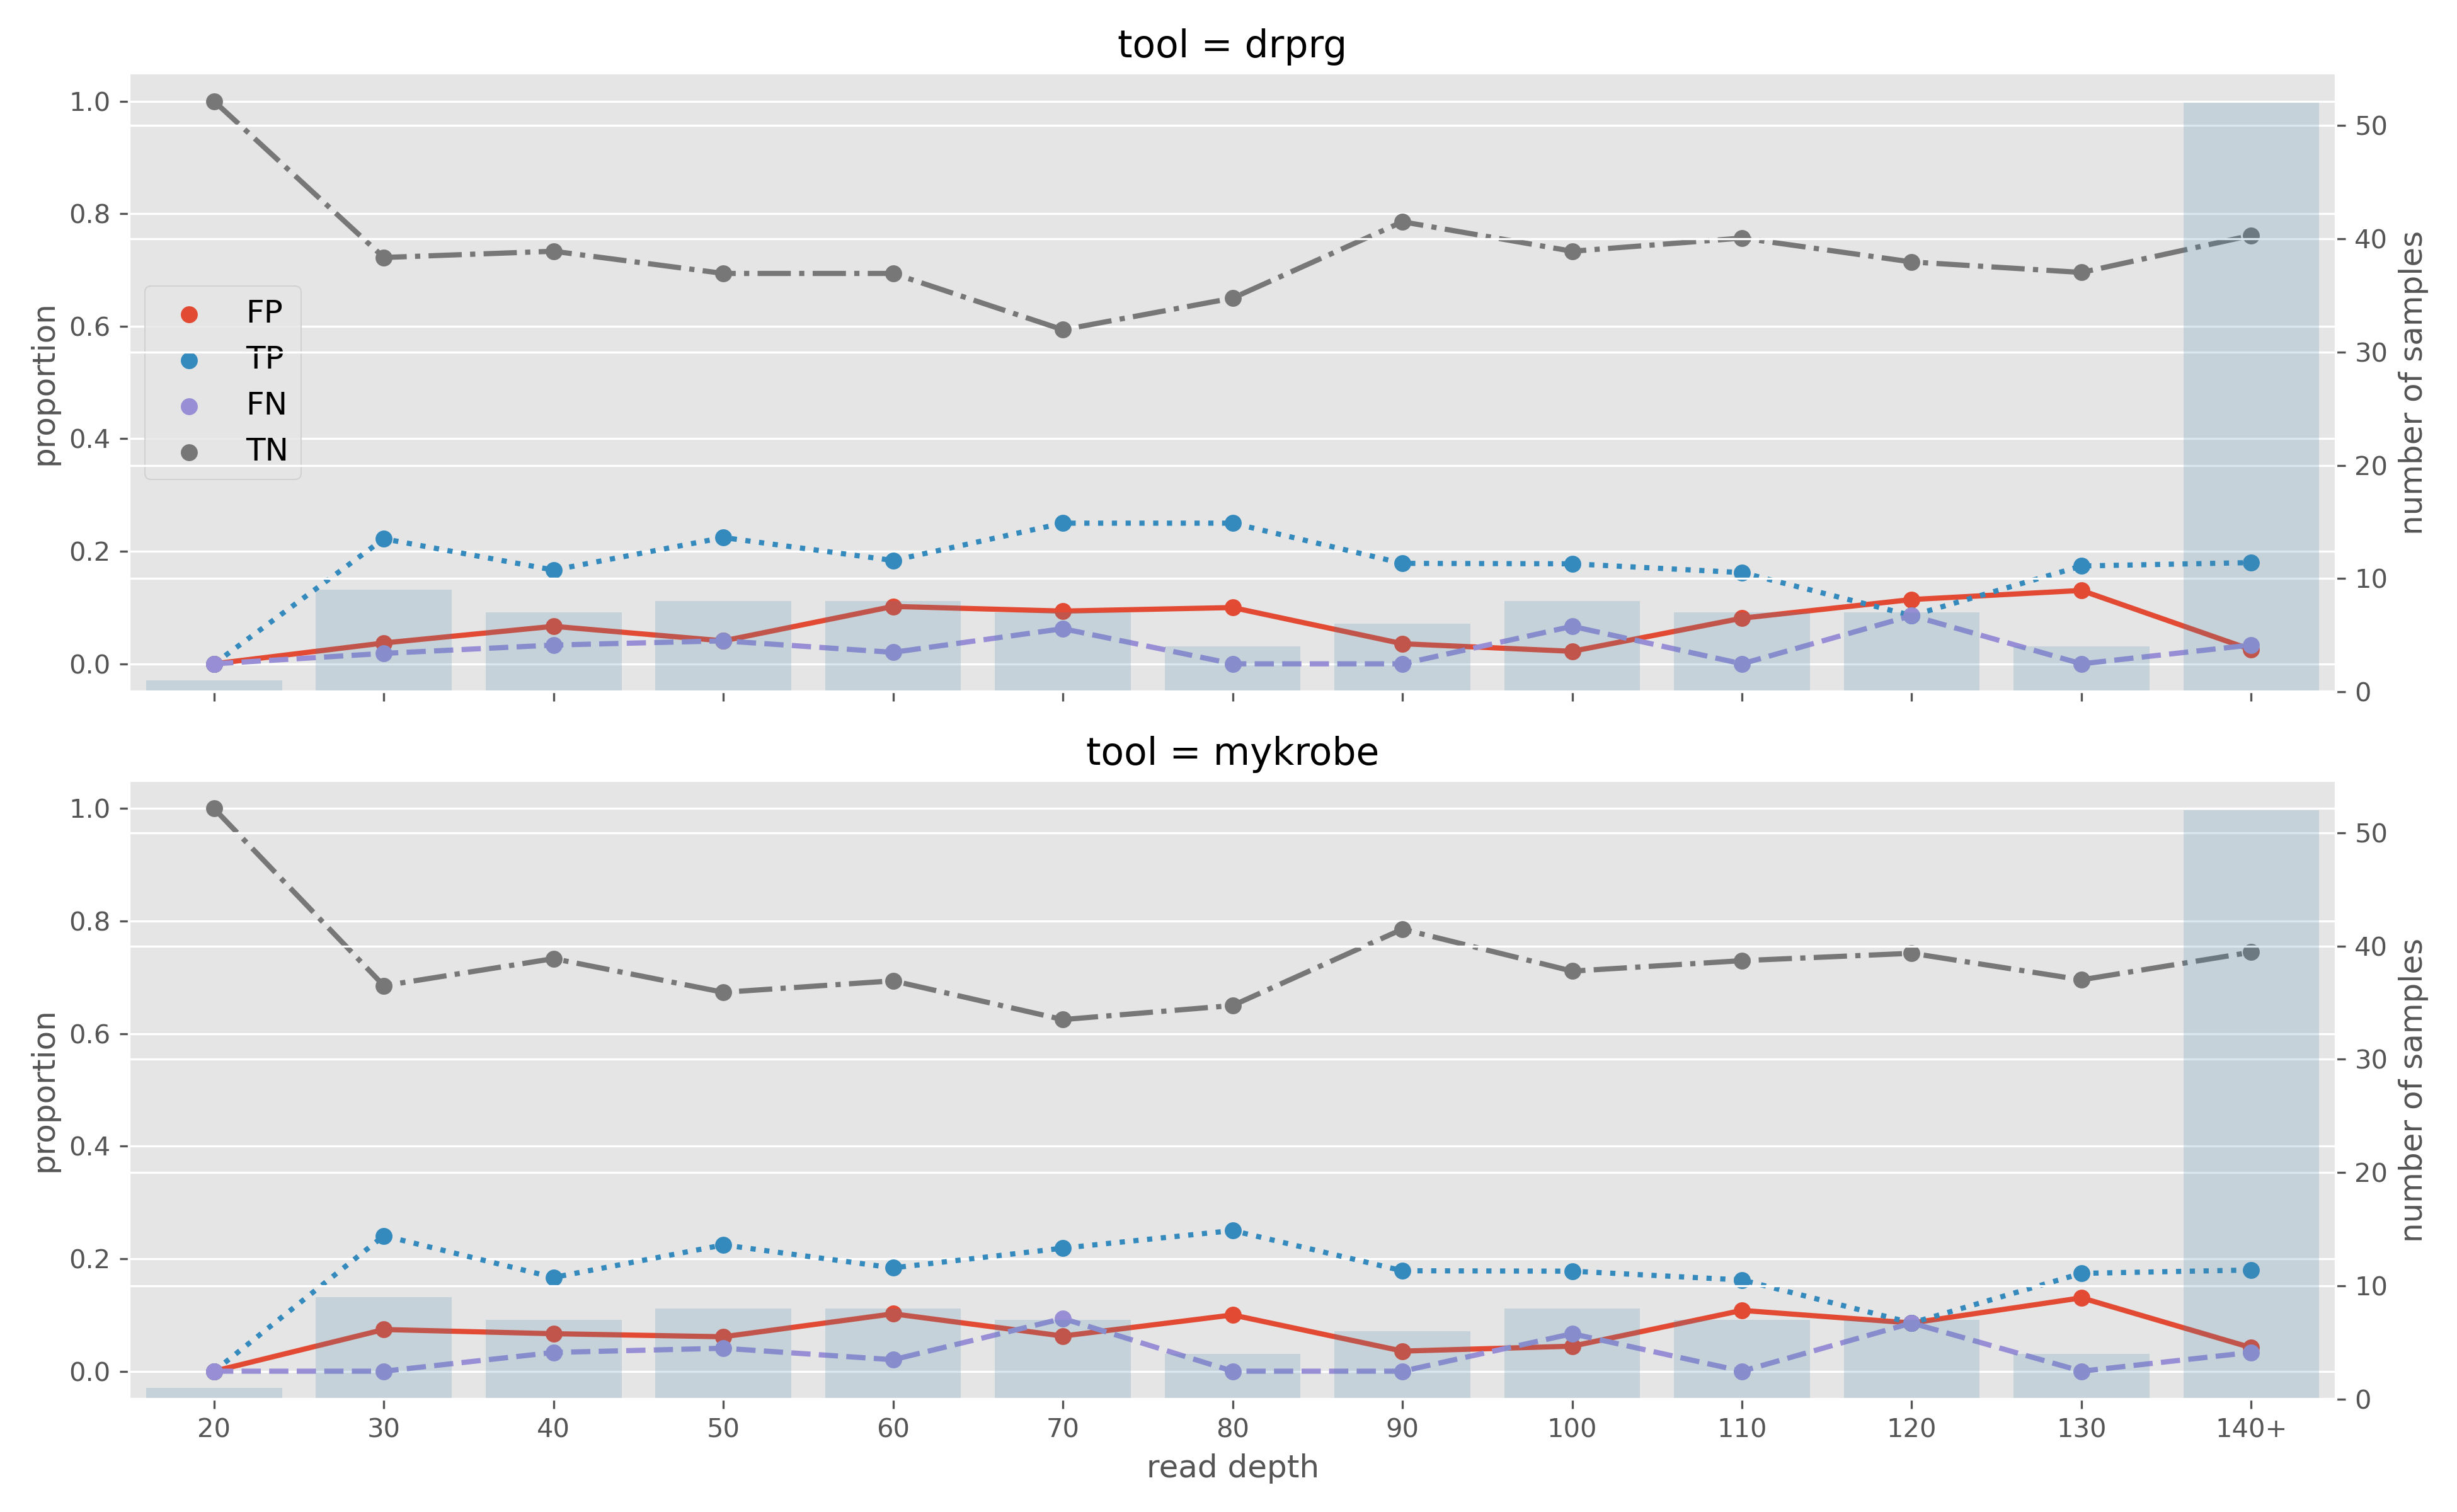
\includegraphics[width=0.90\columnwidth]{Chapter3/Figs/phenotype_coverage.png}
\caption{{Effect of \ont{} read depth on \drprg{} (top) and \mykrobe{} (bottom) drug susceptibility phenotype prediction. Each point indicates the proportion (left y-axis) of classifications of that type at the read depth (x-axis). Read depth is binned such that 40 is all samples with a read depth $\ge40$ and less than 50. The blue bars indicate the number of samples (right y-axis) contained in each bin. FP=false positive (red); TN=true negative (grey); FN=false negative (purple); TP=true positive (blue).
{\label{fig:pheno-covg}}
}}
\end{center}
\end{figure}
%=========================================================================
\section{Detecting off-catalogue mutations}
\label{sec:drprg-discover}

One of the main advantages \drprg{} has over \mykrobe{} is the ability to discover off-catalogue (novel) variants. The reason \drprg{} can call mutations outside of the panel is that it uses \pandora{} as the underlying method for producing predictions from sequencing reads.

The \cryptic{} Consortium have shown that refusing to make predictions in the case where a non-panel variant is discovered in a resistance-associated gene can improve pan-susceptibility prediction \cite{cryptic2018}. However, that work focused only on first-line drugs and did not detail the variants discovered. 

In this section, we aim to assess the novel variant detection capacity of \drprg{} on both Illumina and \ont{} data. While this study is underpowered to make pan-susceptibility predictions, we have a dataset with well-characterised SNPs from \autoref{chap:denovo}. These high-quality variant calls give us a way of determining how many SNPs \drprg{} finds and misses in resistance-associated genes. 

We remove any position in the COMPASS SNPs VCF from \autoref{sec:illumina-var-call} that falls into one of three categories: i) does not occur inside any mutation catalogue gene; ii) not an alternate allele call; or iii) exists in the panel. After this filtering, we have a VCF containing SNPs in resistance-associated genes that do not occur in the panel - referred to as the truth VCF.

We classify the novel SNPs called by \drprg{} against the truth VCF using \vrb{hap.py} - a VCF comparison program developed by Illumina and the Global Alliance for Genomics and Health Benchmarking Team \cite{happy2019}. \autoref{fig:novel-classifications} and \autoref{tab:novel-classifications} show the number of TP, FP, and FN novel SNP calls made by \drprg{} for each drug across all 150 samples. 

From \autoref{fig:novel-classifications} we clearly see \textit{rpoB} contains the most off-panel SNPs. Of particular note is the large percentage of \textit{gyrA} FNs, which leads to a recall of 0.35 for both Illumina and \ont{} in this gene. Upon further investigation, all of these missed calls were filtered out by \drprg{} due to low FRS. Additionally, we see the same scenario when looking at the \textit{ahpC} FNs - which are much higher in \ont{} data. 

Despite the poor recall in \textit{gyrA} and \textit{ahpC}, the precision of novel \drprg{} calls is encouraging. In total, there were two FPs detected in \textit{rpoB} (for both technologies), and one \ont{} FP in \textit{rrs}. This result suggests we can be very confident in the novel SNP calls made by \drprg{}.

\begin{figure}
\begin{center}
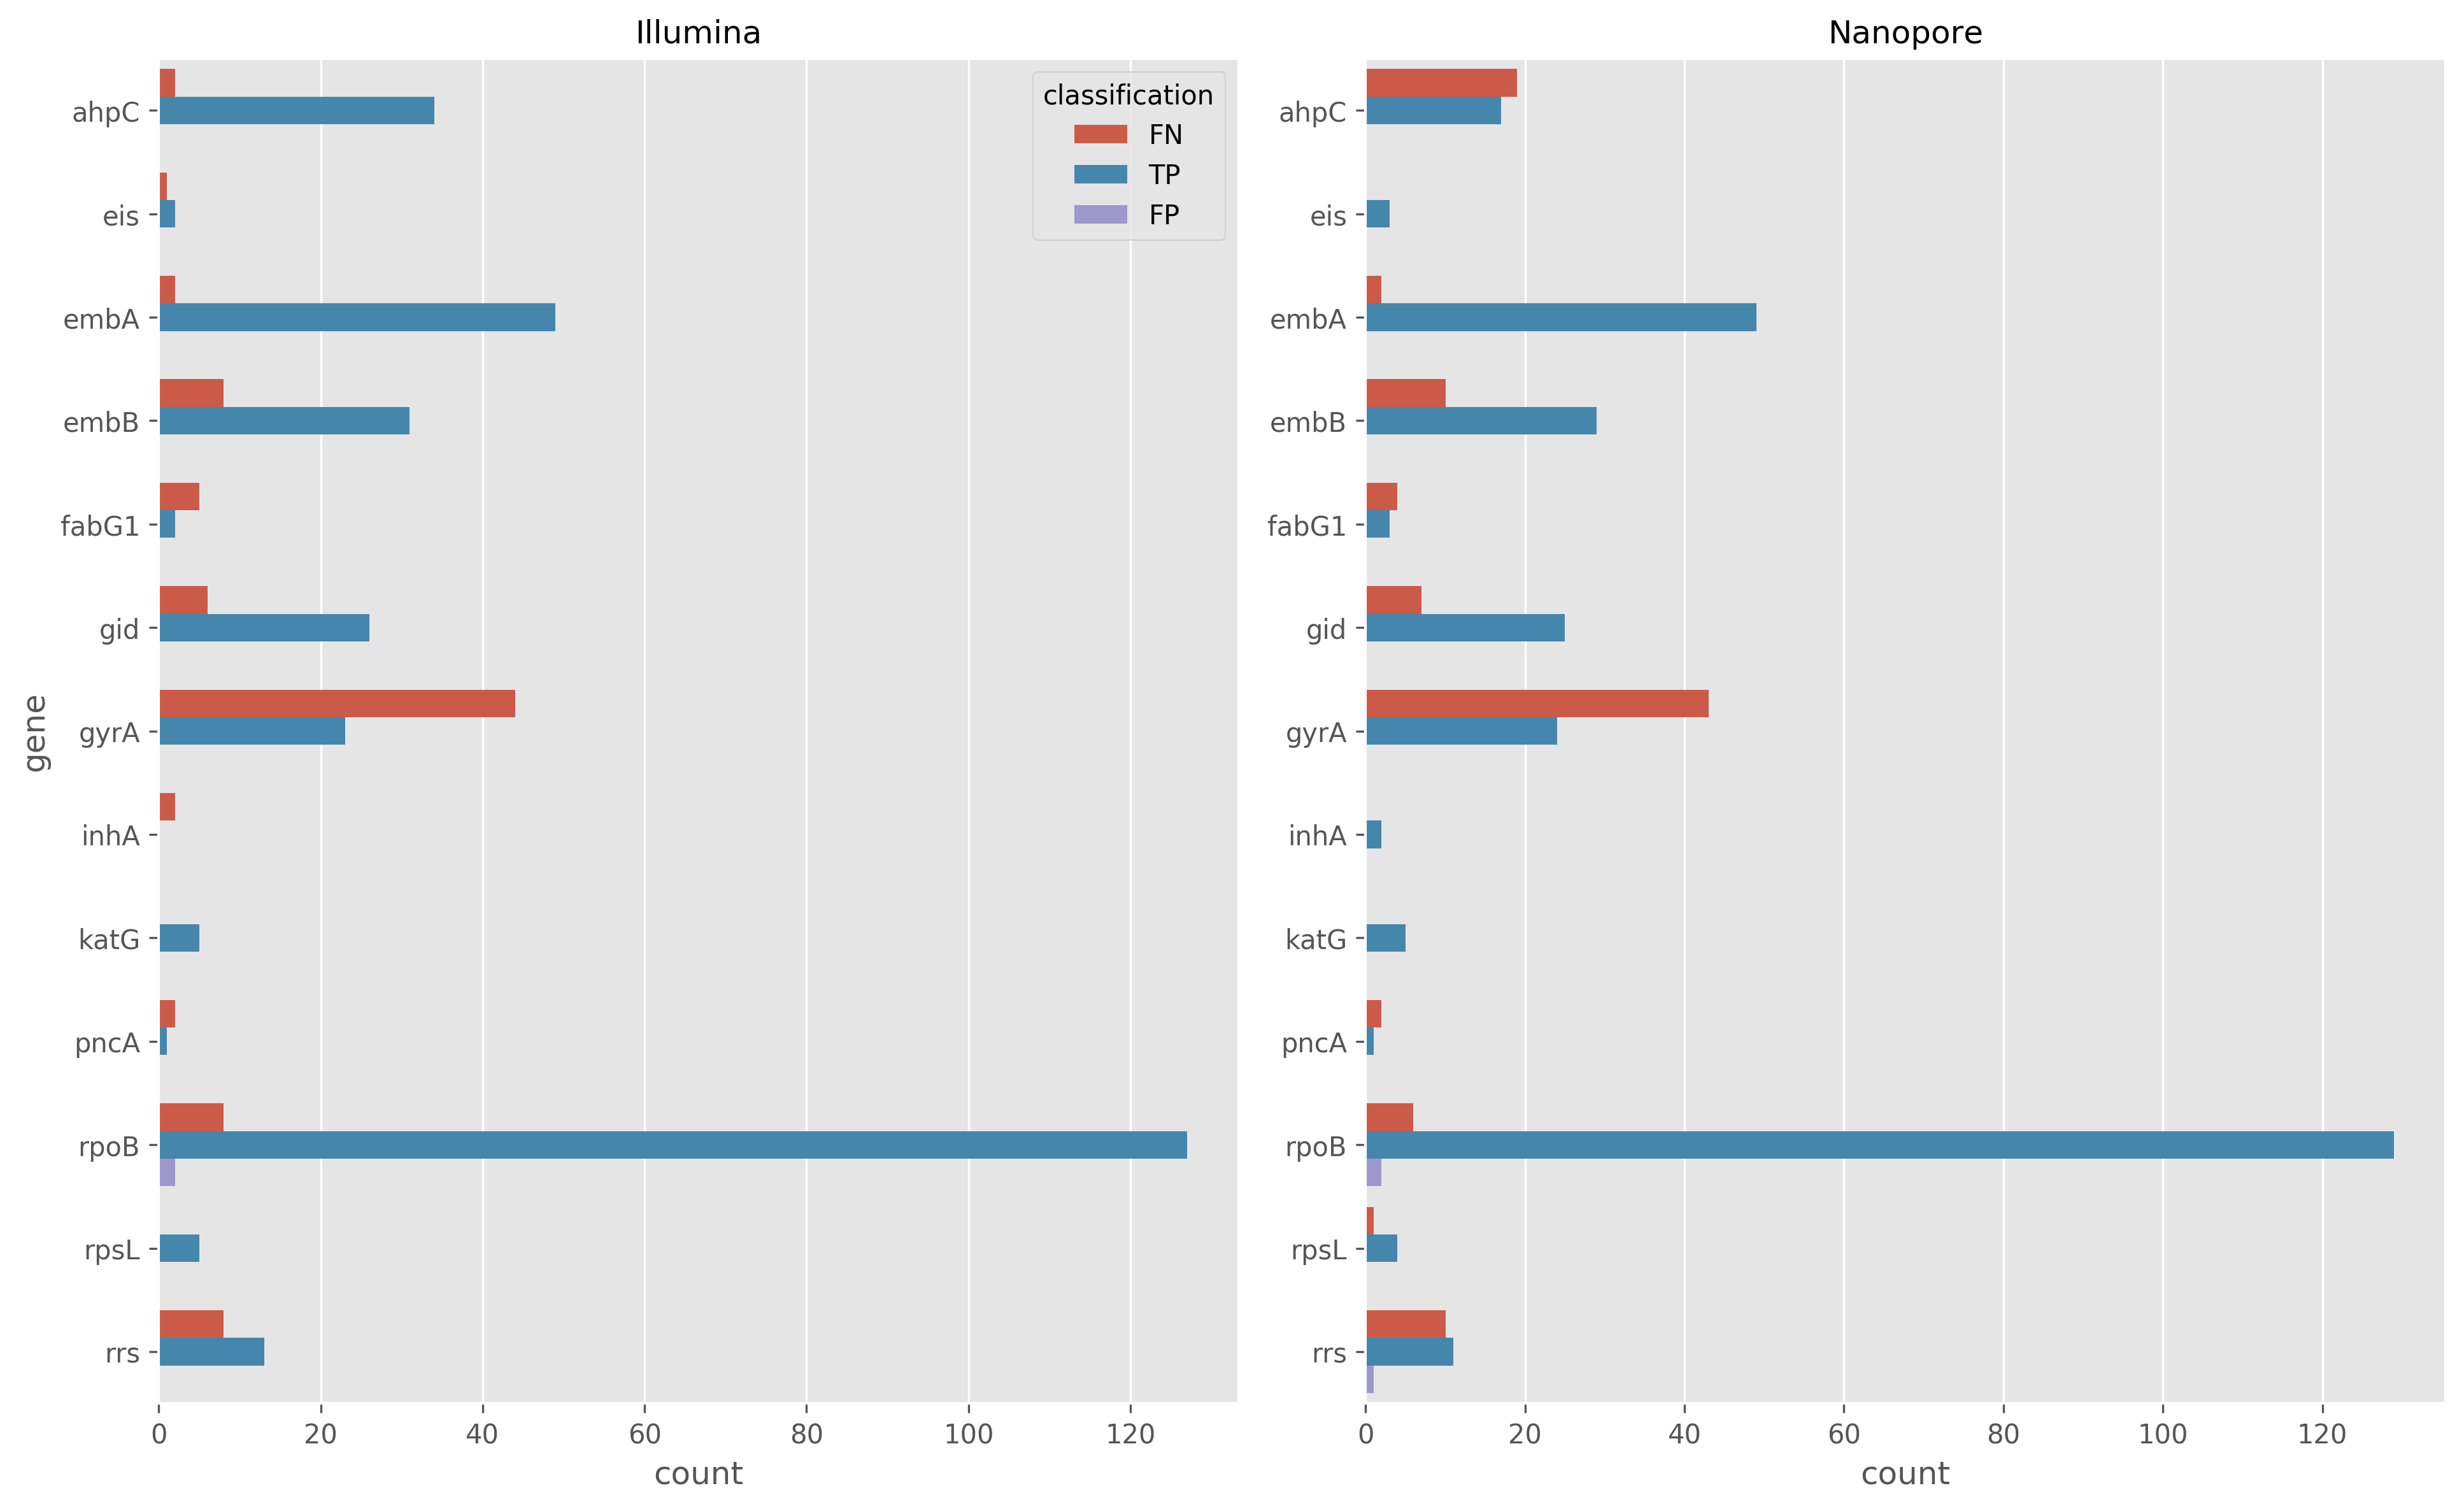
\includegraphics[width=0.90\columnwidth]{Chapter3/Figs/novel_classifications.png}
\caption{{Classifications of novel SNP calls made from Illumina (left) and \ont{} (right) data by \drprg{} in resistance-associated genes (y-axis). Counts (x-axis) are across all samples. TP (blue) - true positive; FN (red) - false negative; FP (purple) - false positive.
{\label{fig:novel-classifications}}
}}
\end{center}
\end{figure}

\begin{table}
\centering
\begin{tabular}{|l|l|c|c|c|c|c|}
\hline
Gene                            & Technology & FN & FP & TP  & Recall & Precision \\ \hline
\multirow{2}{*}{\textit{ahpC}}  & Illumina   & 2  & 0  & 34  & 0.944  & 1.000     \\ \cline{2-7} 
                                & Nanopore   & 19 & 0  & 17  & 0.472  & 1.000     \\ \hline
\multirow{2}{*}{\textit{eis}}   & Illumina   & 1  & 0  & 2   & 0.667  & 1.000     \\ \cline{2-7} 
                                & Nanopore   & 0  & 0  & 3   & 1.000  & 1.000     \\ \hline
\multirow{2}{*}{\textit{embA}}  & Illumina   & 2  & 0  & 49  & 0.961  & 1.000     \\ \cline{2-7} 
                                & Nanopore   & 2  & 0  & 49  & 0.961  & 1.000     \\ \hline
\multirow{2}{*}{\textit{embB}}  & Illumina   & 8  & 0  & 31  & 0.795  & 1.000     \\ \cline{2-7} 
                                & Nanopore   & 10 & 0  & 29  & 0.744  & 1.000     \\ \hline
\multirow{2}{*}{\textit{fabG1}} & Illumina   & 5  & 0  & 2   & 0.286  & 1.000     \\ \cline{2-7} 
                                & Nanopore   & 4  & 0  & 3   & 0.429  & 1.000     \\ \hline
\multirow{2}{*}{\textit{gid}}   & Illumina   & 6  & 0  & 26  & 0.812  & 1.000     \\ \cline{2-7} 
                                & Nanopore   & 7  & 0  & 25  & 0.781  & 1.000     \\ \hline
\multirow{2}{*}{\textit{gyrA}}  & Illumina   & 44 & 0  & 23  & 0.343  & 1.000     \\ \cline{2-7} 
                                & Nanopore   & 43 & 0  & 24  & 0.358  & 1.000     \\ \hline
\multirow{2}{*}{\textit{inhA}}  & Illumina   & 2  & 0  & 0   & 0.000  & -         \\ \cline{2-7} 
                                & Nanopore   & 0  & 0  & 2   & 1.000  & 1.000     \\ \hline
\multirow{2}{*}{\textit{katG}}  & Illumina   & 0  & 0  & 5   & 1.000  & 1.000     \\ \cline{2-7} 
                                & Nanopore   & 0  & 0  & 5   & 1.000  & 1.000     \\ \hline
\multirow{2}{*}{\textit{pncA}}  & Illumina   & 2  & 0  & 1   & 0.333  & 1.000     \\ \cline{2-7} 
                                & Nanopore   & 2  & 0  & 1   & 0.333  & 1.000     \\ \hline
\multirow{2}{*}{\textit{rpoB}}  & Illumina   & 8  & 2  & 127 & 0.941  & 0.984     \\ \cline{2-7} 
                                & Nanopore   & 6  & 2  & 129 & 0.956  & 0.985     \\ \hline
\multirow{2}{*}{\textit{rpsL}}  & Illumina   & 0  & 0  & 5   & 1.000  & 1.000     \\ \cline{2-7} 
                                & Nanopore   & 1  & 0  & 4   & 0.800  & 1.000     \\ \hline
\multirow{2}{*}{\textit{rrs}}   & Illumina   & 8  & 0  & 13  & 0.619  & 1.000     \\ \cline{2-7} 
                                & Nanopore   & 10 & 1  & 11  & 0.524  & 0.917     \\ \hline
\end{tabular}
\caption{Classification of novel SNP calls made by \drprg{} in resistance-associated genes. Counts are across all samples. TP - true positive; FN - false negative; FP - false positive.}
\label{tab:novel-classifications}
\end{table}

\autoref{fig:novel-sample-classifications} illustrates the number of novel calls of different classification on a per-sample basis. It shows that on average, a samples will have 2 novel TP calls and 0 FPs and FNs. 

\begin{figure}
\begin{center}
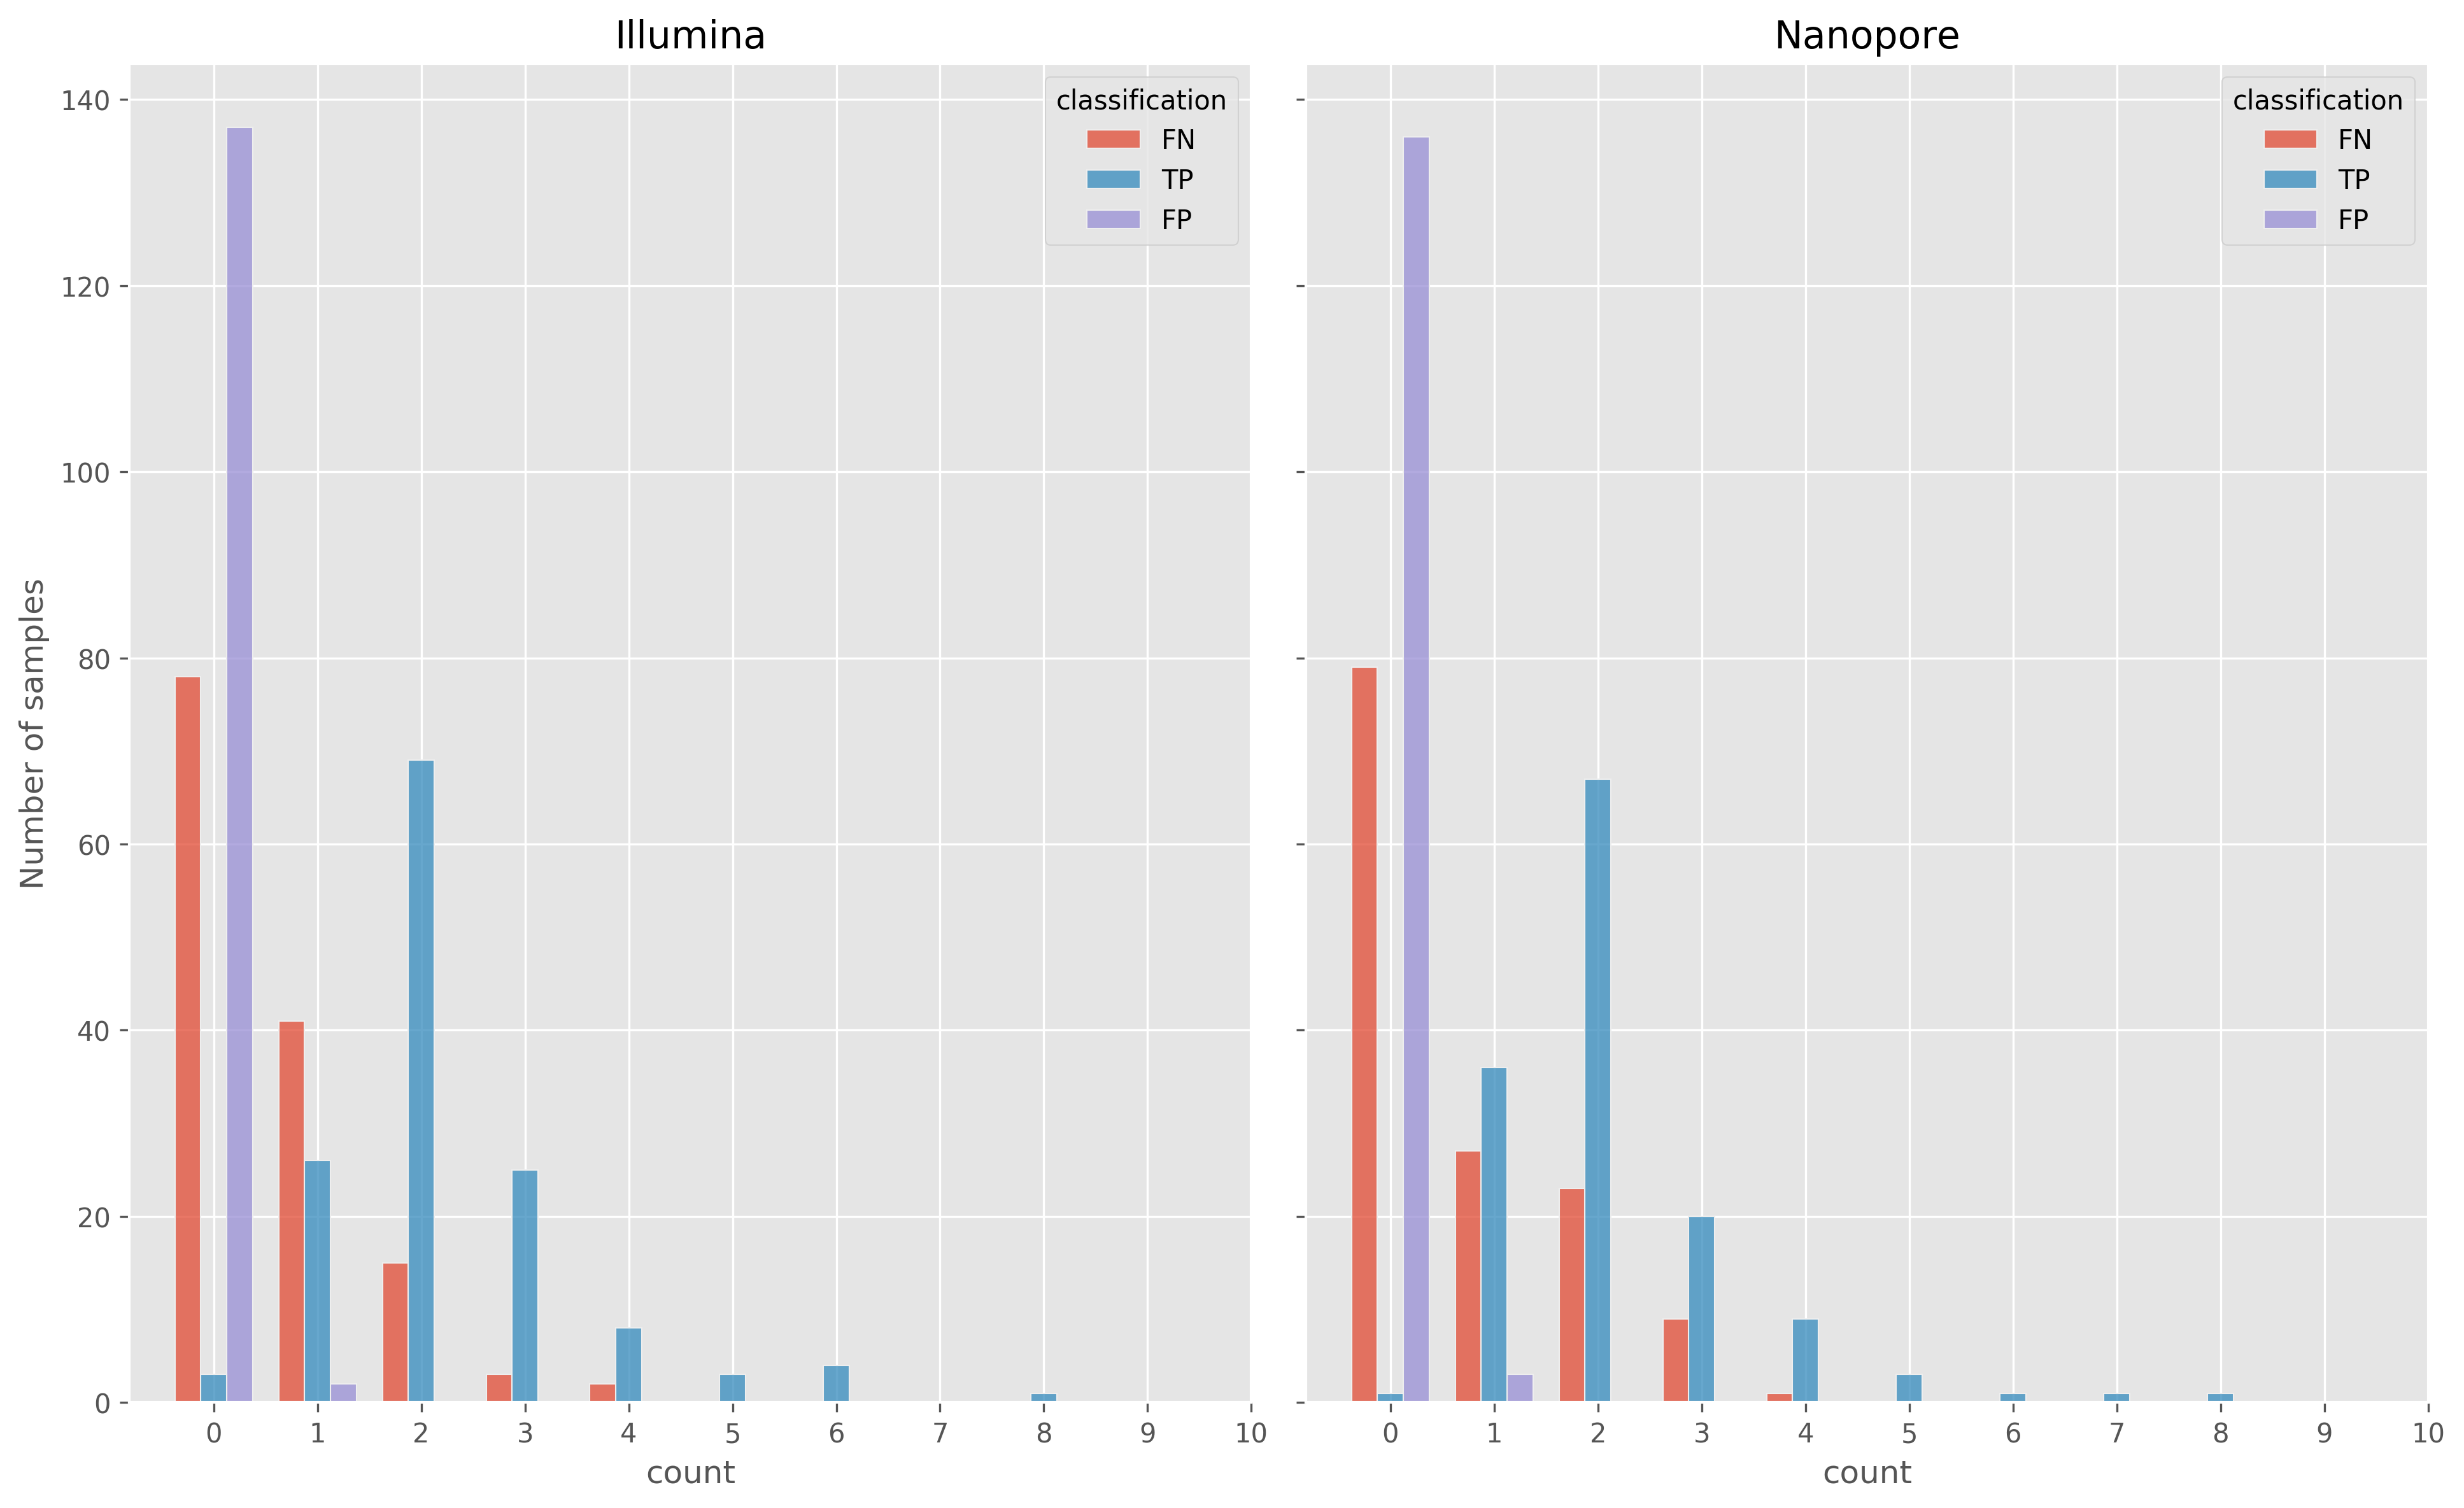
\includegraphics[width=0.90\columnwidth]{Chapter3/Figs/novel_classifications_per_sample.png}
\caption{{Number of novel variants found in resistance-associated genes for each sample. The x-axis indicates the number of classifications of the relevant kind for a sample, and the y-axis is the number of samples with that classification count. The classifications are: TP (blue) - true positive; FN (red) - false negative; FP (purple) - false positive.
{\label{fig:novel-sample-classifications}}
}}
\end{center}
\end{figure}

Having seen that the off-panel SNPs called by \drprg{} are precise, we look at how incorporating this information impacts the AMR predictions. \autoref{fig:pheno-unknown} is the same as \autoref{fig:pheno-concordance}, except with unknown (off-panel) calls included. If we find a novel variant, an unknown prediction is given for the drug(s) associated with that gene. The exception to this is when a known resistance-causing mutation is also found for the respective drug(s), in which case a resistant prediction is made.

Of note in \autoref{fig:pheno-unknown} is the reduced number of missed resistance calls made when we include unknown variants - when compared to \autoref{fig:pheno-concordance}. That is, a call of unknown is our way of indicating to the user that we did not find a \emph{known} resistance-causing mutation; however, we did find a mutation that is not known to be either resistance- or susceptibility-associated.

While we see a reduction in the number of missed resistance calls (FN) when calling unknown variants, the number of definitive susceptibility (TN) calls is also reduced. In particular, ethambutol, rifampicin, and streptomycin see a large number of unknown calls. The large number of unknown calls for rifampicin is not unexpected as \textit{rpoB} (associated with rifampicin resistance) had by far the most novel variants in the above analysis (\autoref{fig:novel-classifications}). Nearly every one of these unknown rifampicin calls relates to synonymous mutations D103D (C309T) and A1075A (T3225C) that are known not to be associated with drug resistance \cite{Jagielski2018}. Likewise, synonymous mutations were also the cause of the bulk of unknown calls for other drugs. However, there were some indel calls found. As our truth VCF only contains SNPs, we cannot assess the validity of these indel calls.

A simple solution for the excessive unknown calls in susceptible samples would include synonymous mutations in the panel as susceptibility-associated.

\begin{figure}
\begin{center}
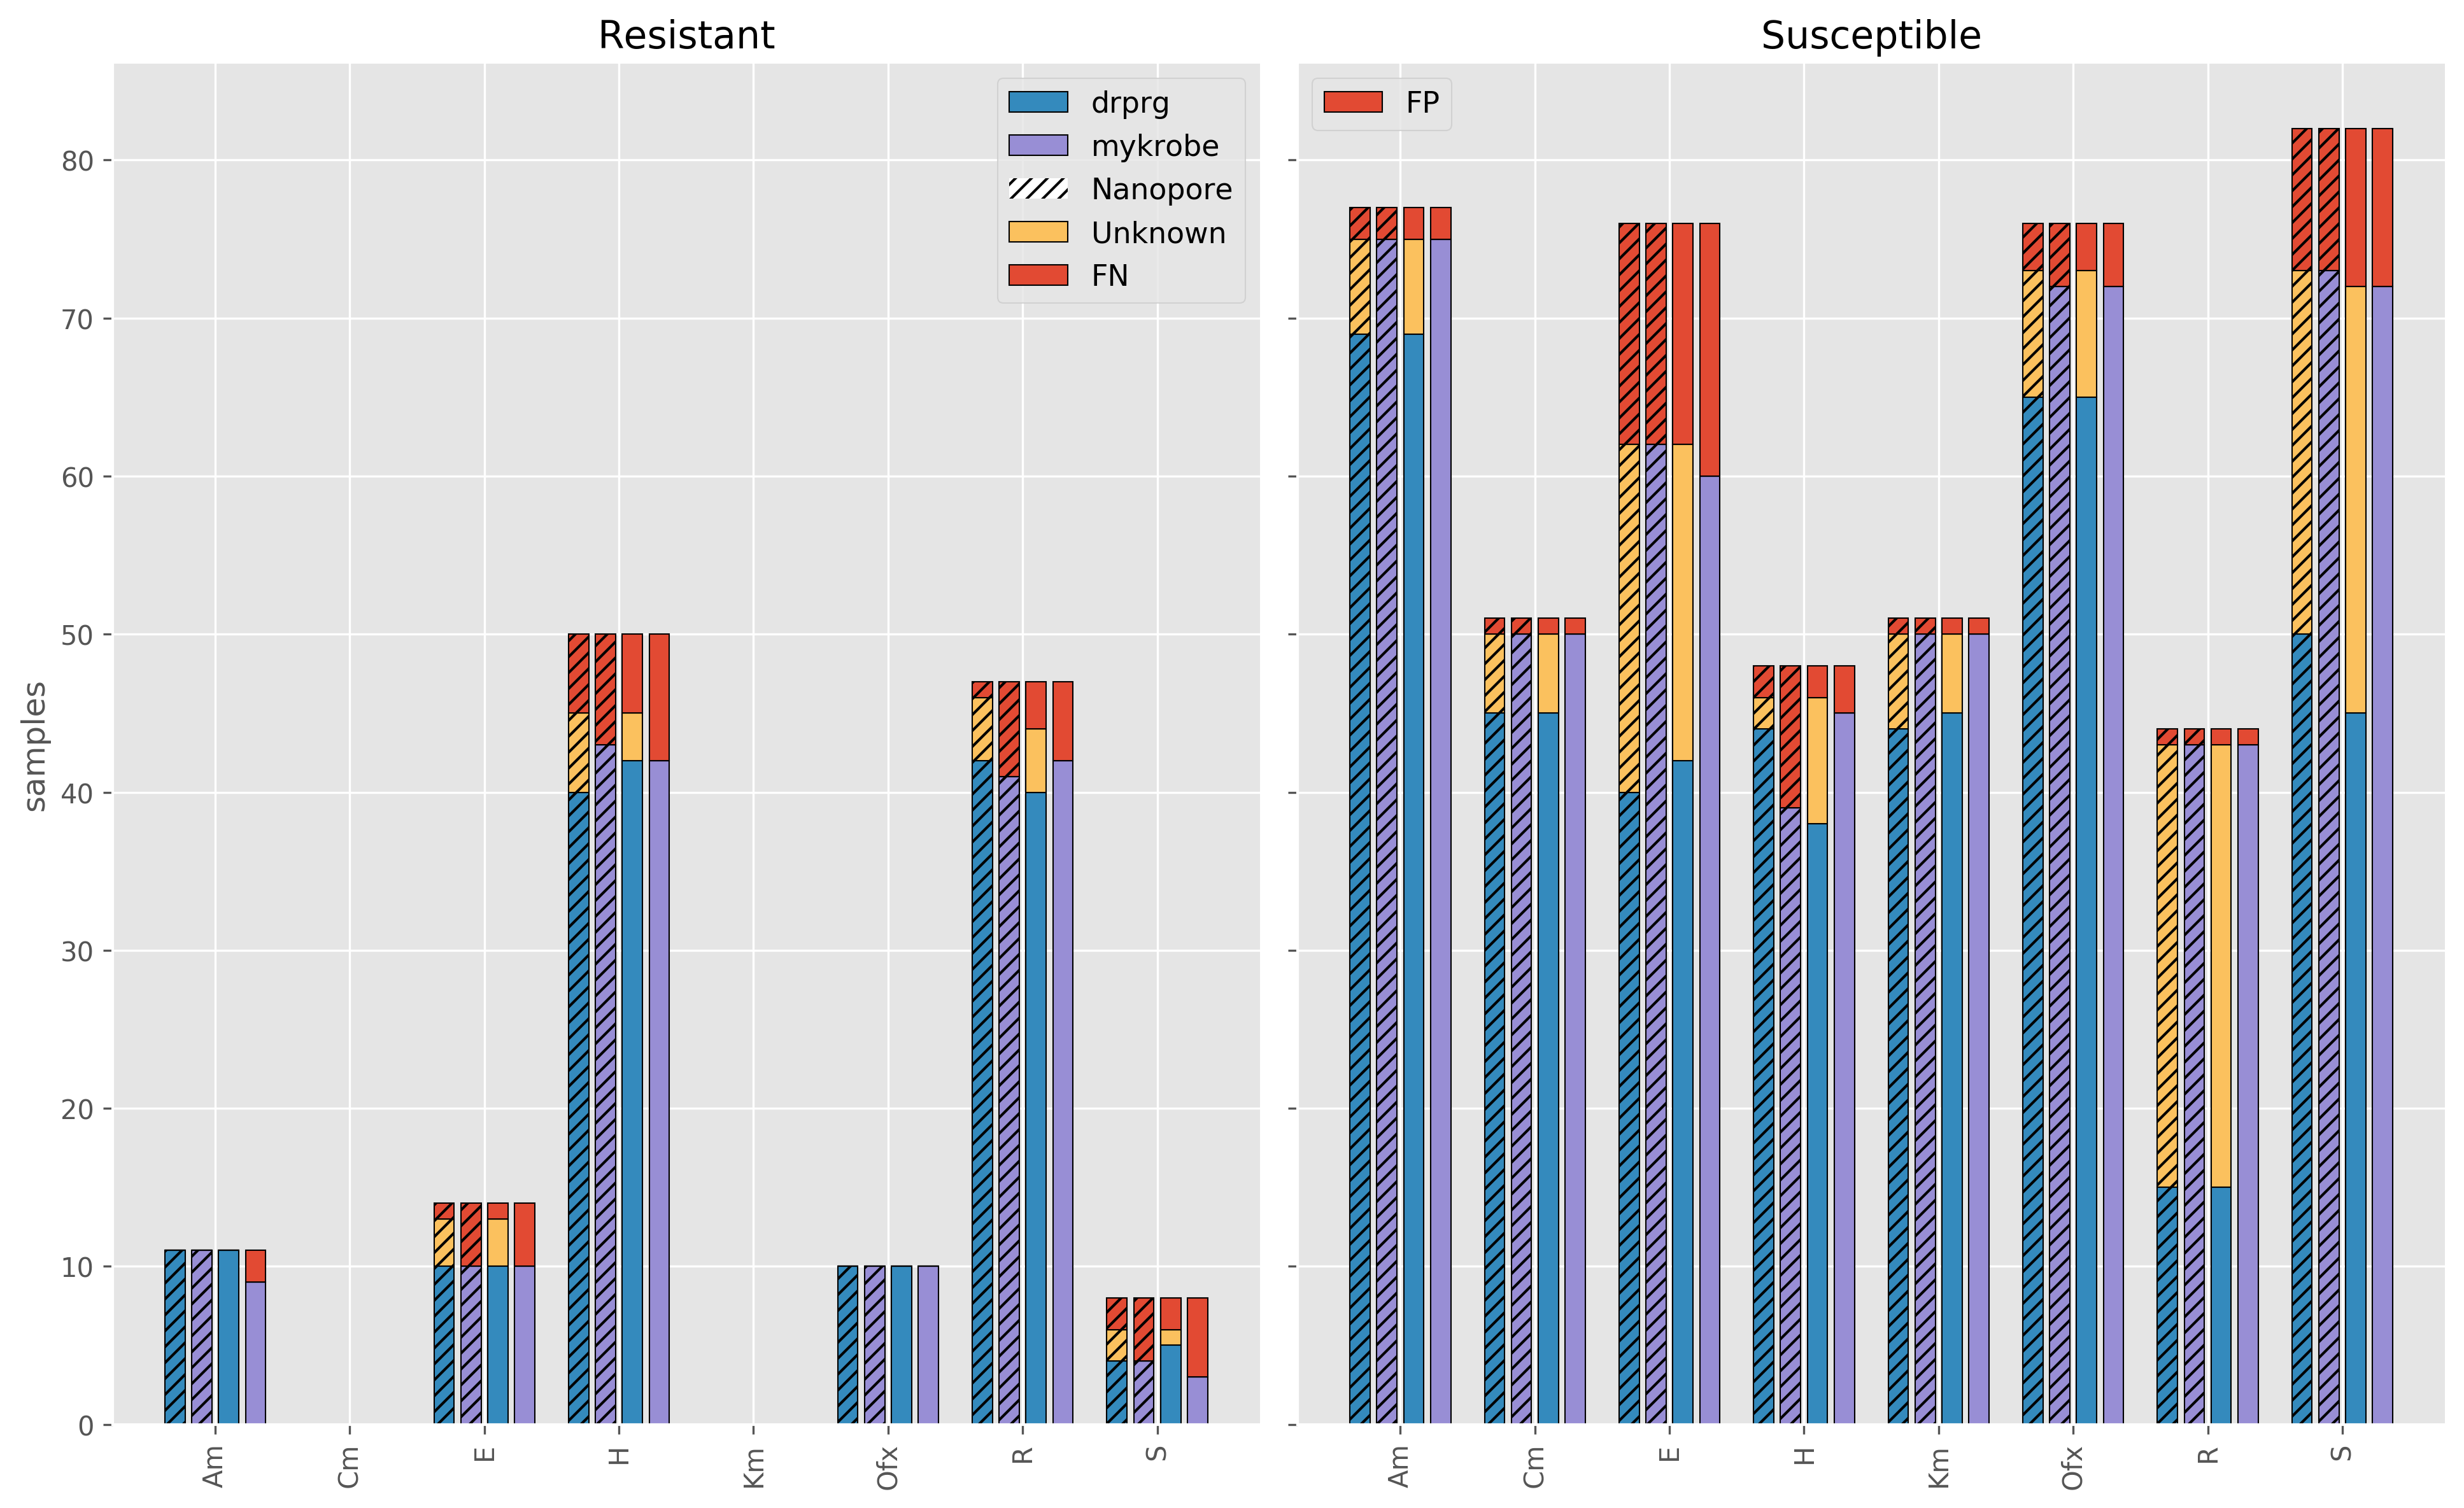
\includegraphics[width=0.90\columnwidth]{Chapter3/Figs/pheno_unknown.png}
\caption{{Number of resistant (left) and susceptible (right) culture-based drug susceptibility testing (DST) phenotypes correctly identified by \mykrobe{} (purple) and \drprg{} (blue) with Illumina (non-striped) and \ont{} (striped) data. The red bars indicate missed (FN) or incorrect (FP) predictions. The yellow bars represent \drprg{} "unknown" calls, which is when there is an off-panel variant found in a gene associated with the respective drug. If there is no resistance-associated variant found for that drug, then an unknown call is made. The x-axis shows the drugs with available phenotype data. E - ethambutol; H - isoniazid; R - rifampicin; S - streptomycin; Km - kanamycin; Am - amikacin; Ofx - ofloxacin; Cm - capreomycin.
{\label{fig:pheno-unknown}}
}}
\end{center}
\end{figure}

\subsection{Summary}

Producing unknown drug resistance predictions based on novel variant calls is a point of difference for \drprg{}. In this section, we have shown that novel variants detected by \drprg{} are precise, but that missed calls require some more work.

We have also shown that we can reduce missed resistance calls by refusing to make predictions for drugs with variants of unknown consequences. However, this currently comes at the cost of fewer susceptibility calls, although an easy fix - incorporating synonymous mutations - has been identified.

%=========================================================================
\section{Discussion}
Illumina WGS has become a standard tool for \mtb{} drug susceptibility testing. Its use is underpinned by a vast number of studies validating the sensitivity and specificity of such predictions, all with similar results \cite{cryptic2018,hunt2019,bradley2015,coll2015,walker2015,kohl2018,phelan2019}. In this chapter, we have provided evidence that \ont{} WGS-based DST can provide predictions consistent with Illumina. We did this by first showing that when comparing Illumina and \ont{} predicted phenotypes to culture-based phenotypes, there is very little difference between the predictions from the two technologies. However, for isoniazid, we do note a higher \ont{} false positive rate (18.8\%) than Illumina (6.2\%) when using \mykrobe{}.

In addition to validating the use of \ont{} for DST, we also developed and evaluated a software tool \drprg{} for the same task. Many programs exist to predict drug resistance from WGS data; however, all have the same underlying limitation: an inability to detect off-panel (novel) mutations. With \drprg{} we have made a first step in removing this limitation from \mtb{} AMR prediction.

\drprg{} is not the first tool to use the concept of genome graphs for AMR prediction. \mykrobe{}, the other tool used in this chapter, uses population genome graphs for genotyping of samples. The underlying method \mykrobe{} uses is Cortex \cite{iqbal2012} - a program that uses coloured de Bruijn graphs for genotyping samples via \denovo{} assembly. Cortex is somewhat of a precursor to \pandora{} - the genome graph method underpinning \drprg{}. However, \pandora{} offers a number of advantages over Cortex (see \autoref{sec:genome-graphs-dst} for a full description of these). Ultimately, the differences mean, theoretically, \pandora{} (\drprg{}) requires less read depth to produce the same information as Cortex (\mykrobe{}) and is much better suited to use with noisy, error-prone \ont{} data. 

When comparing the computational performance of \mykrobe{} and \drprg{}, we found \drprg{} to be faster and more memory efficient for both technologies (\autoref{sec:drprg-comp-perf}).

\noindent
Given the extensive validation of Illumina WGS for DST, with many more samples than we have in this chapter, our intention is not to assert the clinical use of WGS. Rather, we seek to gauge \ont{}'s suitability for WGS-based DST. We first assessed Illumina and \ont{} predictions against "gold-standard" culture-based phenotypic testing in \autoref{sec:pheno-concordance}. This analysis allows an unbiased assessment of the two sequencing modalities, intending to detect any technology-driven differences. As all our samples were sequenced from the same DNA extraction, we know the resistance profile for the underlying data is the same for both technologies. 

\ont{} has been assessed for use in providing AMR predictions previously \cite{bradley2015,hunt2019,phelan2019}, but with single-digit sample sizes. An exception to this is the work by the New York State Department of Health, which used a sample size of 431 \cite{smith2020}. Our results from \autoref{sec:pheno-concordance} are in agreement with all of these previous studies; \ont{} AMR predictions are highly concordant with Illumina when compared to culture-based phenotypes - using our altered parameters from \autoref{app:mykrobe-settings}. This agreement is found for both \mykrobe{} and \drprg{}. As mentioned, the one exception to this was \mykrobe{}'s \ont{} isoniazid predictions, which had a higher false-positive rate compared to the other technology/tool combinations. All of these extra FPs were due to \textit{katG} indel calls in the \ont{} data, which as mentioned, is a systematic problem currently affecting \ont{} \cite{watson2019}. One point of difference between the \ont{} study by Smith \etal{} and ours is that our dataset is from three countries with very different \mtb{} populations, whilst Smith \etal{} use a more homogeneous population from New York state. 

While there is a high level of similarity between predictions from both tools and sequencing modalities, disagreement with the culture-based phenotype is high for some drugs. For example, the ethambutol false negative rate (FNR; 28.6\%) was much higher than previous reports, which generally fall in the 5-10\% range \cite{cryptic2018,hunt2019,smith2020}. However, Smith \etal{} did see an FNR of 20\%. In addition, the positive predictive value (PPV; also known as precision) was 41.7\%, again, much lower than previous studies. However, all FP predictions were made due to a non-synonymous mutation at codon 306 in \textit{embB}.  We saw consistent support for the presence of these FP mutations on all technologies and tools, and multiple previous reports have strongly linked this mutation to ethambutol resistance \cite{Maningi2017,Srivastava2009,Brossier2015}. To further reinforce the possibility of an incorrect culture-based phenotype in these cases, where line probe assay phenotypes were available for ethambutol, most of these were inconsistent. Indeed, sequencing of the resistance-associated genes is now recommended over culture-based phenotyping for ethambutol \cite{who2018technical}. 

We also see similarly poor performance for both PPV and FNR in streptomycin when compared to other studies. Our isoniazid FNR of 14-20\% is also higher than previous work, but not by as much as streptomycin and ethambutol. In almost all of these errors, we again see discrepant LPA phenotypes and strong evidence for mutations previously linked to drug resistance, but not in our panel. These discrepancies raise the ongoing need for a curated panel of known mutations and their impacts on susceptibility. Additionally, they highlight the imperfection of culture-based phenotyping, which has been discussed elsewhere \cite{walker2015, who2018technical,cryptic2018}.

The main limitation for this section of the chapter is the number of resistant samples. Although there was 50 isoniazid- and 47 rifampicin-resistant isolates, the other drugs had no more than 15 samples representing. The low number of resistant samples is reflected in the breadth of confidence intervals for all drugs. However, combining this dataset with Smith \etal{} \cite{smith2020} would provide an increase in the matched Illumina/Nanopore data with susceptibility profiles for all drugs.

\noindent
As \mykrobe{} has been extensively validated on large datasets with Illumina \cite{bradley2015,hunt2019}, using it as a truth to compare \ont{} to provides further validation for \ont{}'s use for AMR prediction. The added advantage to such an approach on our dataset is that we can get a sense of the performance of \drprg{} and \mykrobe{} \ont{} for all drugs for which \mykrobe{} provides predictions. As culture-based phenotypes were not available for all drugs and samples, this gives us additional insight. We performed this analysis in \autoref{sec:geno-concordance} and found \mykrobe{}'s \ont{} predictions to be highly concordant with those from Illumina. There were only eight missed resistance calls, seven of which were minor resistance calls on Illumina. We attempted to allow minor resistance calls for \ont{}, but this lead to every sample being predicted as resistant to isoniazid and pyrazinamide due to false heterozygous indel calls in \textit{katG} and \textit{pncA}. Of the false-positive calls made by \mykrobe{} on \ont{} data, half were due to indel calls in \textit{katG}, while the other half are quite likely errors on behalf of Illumina due to filtering.

When comparing the \drprg{} predictions to \mykrobe{} Illumina profiles, we see somewhat similar results. As with \mykrobe{} \ont{} errors, almost all \drprg{} errors were due to indel calls in \textit{katG} and \textit{pncA}, while the rest were most likely Illumina errors as mentioned above. 

Taking the analyses in \autoref{sec:pheno-concordance} and \autoref{sec:geno-concordance} together, it is clear that one of the main limitations of \drprg{} is faulty indel calls. Indeed, on many occasions in this thesis, we have stated this is a known systematic issue of \ont{} \cite{watson2019}. However, we believe this is a problem worth careful consideration as it has a big impact on isoniazid and pyrazinamide resistance - both first-line \mtb{} drugs. We discuss future directions for improving on this limitation of \drprg{} in \autoref{sec:indel-dst-fw}.

\noindent
Having established \ont{}-based AMR predictions for \mtb{} are comparable to Illumina, we next looked at whether the \ont{} performance is dependent on the read depth available. In 2017, Votintseva \etal{} concluded that the accuracy of \ont{} for providing real-time AMR predictions for \mtb{} was dependent on "deep coverage" \cite{Votintseva2017}. While four years may not seem like a long time in science, in the world of \ont{} sequencing, it is an age. Technological advances in \ont{} sequencing happen so quickly that regular benchmarks are warranted (but tedious). Given that our dataset has samples with read depth ranging from 29-150x, in \autoref{sec:dst-covg} we assessed whether there was a higher proportion of misclassifications at lower depths. As \autoref{fig:pheno-covg} very clearly shows, there is no evidence in our dataset that read depth has any influence on AMR predictions. To our knowledge, this is the first time such an analysis correlating read depth and classifications has been presented. The consequences of this finding are quite important. Being able to obtain reliable predictions from low-coverage data saves time and money by not having to re-sequence low-yield \ont{} runs, something which is common when multiplexing samples on the one flowcell.

\noindent
Although there are many \mtb{} AMR prediction tools available, \drprg{} is the first to recognise novel variants. When an off-panel variant is found in a gene associated with drug resistance, the prediction for the drug(s) it impacts is designated "unknown". While this is not the first study to investigate the impact of unknown variants on predictions \cite{cryptic2018,hunt2019}, it is the first to provide the functionality to do so in a single program.

We used the Illumina variant calls from COMPASS in \autoref{sec:illumina-var-call} to curate a list of off-panel SNPs we expect to find for each sample. As would be expected from the \pandora{} validation in \autoref{sec:map-var-calls}, \drprg{} produces very precise novel SNP calls, but has some room for improvement for SNP discovery (\autoref{fig:novel-classifications}). Many of the novel SNPs were synonymous mutations, highlighting a gap in the panel construction step of \drprg{} (\autoref{sec:drprg-index}) - where we do not incorporate such mutations unless they are explicitly provided. In addition, the higher number of FN novel SNPs in \textit{ahpC} and \textit{gyrA} were caused by \drprg{} filtering them out for low fraction of read support. Given that these SNPs did not show signs of heterozygosity in the COMPASS VCFs, this warrants further investigation into why were are seeing considerable read depth on multiple alleles at these sites.

When unknown predictions for a drug are interpreted as a refusal to make a prediction - as in \cite{cryptic2018} and \cite{hunt2019} - we see a noticeable decrease in the number of missed resistance calls for ethambutol, isoniazid, rifampicin, and streptomycin. That is, rather than erroneously calling those samples susceptible, we raise the presence of an unknown mutation, indicating further testing is warranted. On the other hand, the same approach needlessly classifies susceptible samples as unknown. In particular, the same drugs mentioned above would have a sizeable proportion of susceptible isolates called unknown. Although, as mentioned, many of these unknown predictions are synonymous mutations, so these unnecessary unknowns are likely easy to fix.

A limitation to our novel variant analysis was the absence of novel indel call validation. Indels are an especially important determinant of resistance for pyrazinamide and isoniazid, so future work should focus on generating a high-quality truth set for the evaluation of \drprg{} indels.

%=========================================================================
\section{Conclusion}
In conclusion, the work in this chapter provides validation that WGS-based drug resistance predictions from \ont{} data are consistent with those from Illumina. Given the extensive validation of Illumina for \mtb{} AMR prediction in clinical settings, the congruence we present suggests that \ont{} can also be used in the same setting. However, further validation on a more extensive dataset is warranted. 

We also describe and evaluate a new method for AMR prediction using genome graphs - \drprg{}. We showed that predictions from \drprg{} are consistent with those from \mykrobe{} - and better for some drugs - whilst being faster and more memory frugal. Importantly, \drprg{} is the first \mtb{} AMR prediction tool with the option to return an unknown prediction in cases where novel variants are found in resistance-associated genes. Furthermore, the novel variants discovered by \drprg{} are precise and lead to a reduced number of missed resistance calls.

%=========================================================================
\section{Future work}

\subsection{Mutation catalogue improvement}

The panel (catalogue) describing the consequence of each mutation is a vital component of any AMR prediction program and can be the primary point-of-difference between tools \cite{hunt2019}. For the work in this chapter, we used the default \mykrobe{} panel for \drprg{}. However, there are two changes to the \drprg{} panel that we would like to incorporate in future work: synonymous mutations and including variants from a new WHO catalogue.

\subsubsection{Synonymous mutations}

As we saw in \autoref{sec:drprg-discover}, many of the off-catalogue mutations signalled as unknown predictions were synonymous mutations - i.e., they lead to no amino acid change. To our knowledge, there have been no synonymous mutations linked to \mtb{} drug resistance. As such, adding the ability for \drprg{} to inherently allow such mutations, without raising them as unknown, would lead to dramatically less unknown predictions - especially in \textit{rpoB} (rifampicin).

\subsubsection{WHO panel}

The WHO has recently released a curated catalogue of \mtb{} mutations and their associated impact on drug susceptibility \cite{whopanel2021}. Incorporating such a panel into the one used in this chapter would likely improve the ability to detect resistance. Indeed, the inclusion of known susceptibility-associated mutations into the \drprg{} helped reduce the novel classifications.

As an example, in \autoref{sec:pheno-concordance}, we saw a streptomycin FN classification, where \drprg{} had called an unknown mutation. This unknown mutation represents the amino acid change K88M in \textit{rpsL}. However, this mutation is listed as resistance-associated in the WHO catalogue and has been linked to streptomycin resistance \cite{Smittipat2016}.

The apparent first improvement would be to incorporate all WHO variants associated with resistance that are not already in our panel. Further work could look to include the mutations listed as "uncertain significance" in a meaningful way.

\subsection{Low read depth samples}

In \autoref{sec:dst-covg} we showed that read depth has no noticeable impact on AMR predictions. However, the lowest depth sample in this chapter has 29x read depth. This depth threshold was a conscious decision made in \autoref{sec:ch2-qc}, where we excluded any sample with less than approximately 30x read depth from further analysis. Thus, there are 33 samples in our full dataset that have \ont{} read depth between 5 and 30x. For those with culture-based phenotype information, we could repeat the analysis in \autoref{sec:dst-covg}. We would then have an even more fine-grained idea of where the \ont{} read depth limits are for reliable AMR predictions.

\subsection{Validation on a larger datasets}

Smith \etal{} recently published a dataset of 431 \mtb{} isolates with matched \ont{} and Illumina sequencing \cite{smith2020}. As they are from the New York State Department of Health, these samples also have gold-standard DST information for eight drugs we provide predictions. Importantly, they have phenotype information for pyrazinamide, one drug we did not have sufficient data for in this chapter. Combining this dataset with ours would give us a very good \ont{} validation set and provide improved confidence in the false-positive and -negative rates. 

In addition to improving the validation numbers for \ont{}, we could also provide vastly improved validation for \drprg{} Illumina predictions by running on previous large cohort studies such as \cite{cryptic2018,hunt2019,phelan2019}. Given that we know \ont{} and Illumina predictions from \drprg{} are consistent, validating Illumina on such large and diverse datasets would be extremely informative overall.

\subsection{Indel calls}
\label{sec:indel-dst-fw}
Indels are important variants for \mtb{} drug resistance. In particular, any frameshift in \textit{katG} or \textit{pncA} leads to isoniazid or pyrazinamide resistance respectively \cite{miotto2017}. Perhaps the limitation we rue the most from \autoref{chap:clustering}, and this chapter, is the lack of in-depth indel analysis. These mutation types have appeared as error causes for several tools and drugs in this chapter. Thus, indel-calling must be assessed in future work.

To properly evaluate and improve indel calls, we need a trustworthy set of expected variants. In \autoref{sec:drprg-discover} we only investigated novel SNP calls made by \drprg{}, as we already had a reliable truth set from \autoref{chap:clustering}. Our proposed method for gathering such a truth panel of indels would be to run Clockwork (\url{https://github.com/iqbal-lab-org/clockwork}; manuscript in preparation) on all samples. Clockwork calls variants with \vrb{samtools} and Cortex and integrates them for a high-quality, filtered set of SNPs and indels.

\ont{}'s ability to produce reliable indel calls is still poor; recent benchmarks show F1-scores around 50\% \cite{clairvoyant2019}. The overwhelming cause of indel errors from \ont{} is around sites with homopolymer deletions. In \autoref{chap:tubby} we will attempt to mitigate these errors by training a \mtb{}-specific \ont{} basecalling model.

\subsection{Lineage classification}

One noticeable feature lacking from \drprg{}, when compared to other tools such as \mykrobe{} and TB-Profiler \cite{phelan2019}, is the ability to identify the lineage of a sample. This functionality is easily added to \drprg{} by building a \prg{} containing only small regions around lineage-defining variants \cite{Shitikov2017,Rutaihwa2019,stucki2016}. Such a \prg{} would only need the wild-type allele and an alternate allele that defines a given lineage. Identifying the lineage would be as simple as matching the genotypes across these sites to the lineage from a lookup table.

\subsection{Other species}

While the initial development of \drprg{} has focused solely on \mtb{}, there is no reason it should be exclusive to that species. All that is needed to adapt it for another species is a panel of variants, a reference genome and annotation. Or, as was done in \autoref{sec:drprg-index}, a prebuilt \prg{} from species representatives. \mykrobe{} also provides inbuilt panels for \textit{S. aureus} and \textit{Shigella sonnei}, so beginning with these species and validating on the same data would be the logical first step. 

The main challenge when adapting to other species is how to allow gene presence/absence detection, which is a mechanism of resistance detected by \mykrobe{} for \textit{S. aureus} \cite{bradley2015}. As \pandora{} outputs a consensus sequence for each \emph{present} locus, all that would be required is investigating incorrect gene presence/absence and determining if default parameters need to be altered.

%=========================================================================
\section{Availability of data and materials}

\drprg{} is open-source and freely available under an MIT license at \url{https://github.com/mbhall88/drprg}. The pipelines and scripts used in this chapter are available at \url{https://github.com/mbhall88/head_to_head_pipeline/tree/master/analysis/resistance_prediction}. All analyses were run using the workflow management program \vrb{snakemake} \cite{snakemake2021}. All figures were generated using the Python libraries \vrb{matplotlib} \cite{matplotlib} and \vrb{seaborn} \cite{seaborn} - \autoref{fig:available-dst} was generated using \url{https://github.com/jnothman/UpSetPlot}.

\towrite[inline]{availability of the data if it has been deposited prior to submission}